\section{Introduction}
\label{sec:ch3-introduction}
We model birth-weight risk using a tree-based, nonparametric approach while still modeling the full spectrum of birth-weight outcomes, we focus primarily on gradients of increased LBW risk among possible predictors. Birth-weights are first grouped into quantile-defined categories so the tree can detect subtle shifts in risk across the finer LBW region, providing a more granular view. Because all factors potentially effect birth weight, our goal is to pinpoint combinations of predictors that consistently mark subpopulations with an elevated LBW incidence. 

To avoid "double dipping," or using the same observations to both fit the model and set its prior, we derive LBW quantile cut points and subsequently construct the Dirichlet hyperparameters from the \emph{previous} year's data (2020) and apply them unchanged to the 2021 dataset. Figure~\ref{fig:alphavec} shows the resulting prior vector \(\boldsymbol\alpha\). The left-panel shows full model's expected proportion of observations in both NBW and LBW categories, and the right-panel shows the LBW-only model's uniform prior due to the 10 LBW deciles. Year-to-year, the birth-weight distributions are remarkably stable at the national level, making 2020 a suitable proxy for 2021.

Seven dichotomous maternal-infant predictors maternal race (\texttt{mrace15}), smoking during pregnancy (\texttt{cig\_0}), marital status (\texttt{dmar}), maternal age (\texttt{mager}), education (\texttt{meduc}), adequacy of prenatal care (\texttt{precare5}), and infant gender (\texttt{sex}) are given to CART, searching recursively for the largest improvement gain. To confirm stability and reliability of the split predictors we will create a 10,000 bootstrap ensemble and compare the variable selection and stability across the trees. This will be further elaborated on in Section~\ref{sec:ch3-comparison-depth}. 

\section{Constructing the Informed Prior}
\label{sec:ch3-prior}

\subsection{Quantile Cut Points \& Informed Prior from 2020 Data}
\label{sec:ch3-cutpoints}
All birth weights less than or equal to the threshold of 2.5 kg are divided into ten deciles comprising the 10\% quantiles mentioned earlier. The LBW-region then smoothly transitions from "extremely low" (lowest 10\%) to "moderately low" (highest 10\%), and pool all NBW observations into the eleventh category denoted as \texttt{counts\_above\_2.5kg}. The large NBW group in the full model allows us to see how this dominant category influences tree splits and variable selection. Under different model scopes, the full and LBW-only model contrasts the focus of the models. The LBW-only model centers its attention around variation \emph{within} the LBW-region in Section~\ref{sec:ch3-comparison}.

From the 2020 proportions we construct the Dirichlet prior, \(\boldsymbol{\alpha} = (\alpha_1, \dots, \alpha_K)\). In Figure~\ref{fig:alphavec} the priors show the strength in NBW under the full model and the uniform prior under the LBW-only models across all categories. 

\begin{figure}[H]
    \centering
        \subfloat[\centering Full model informed prior]{{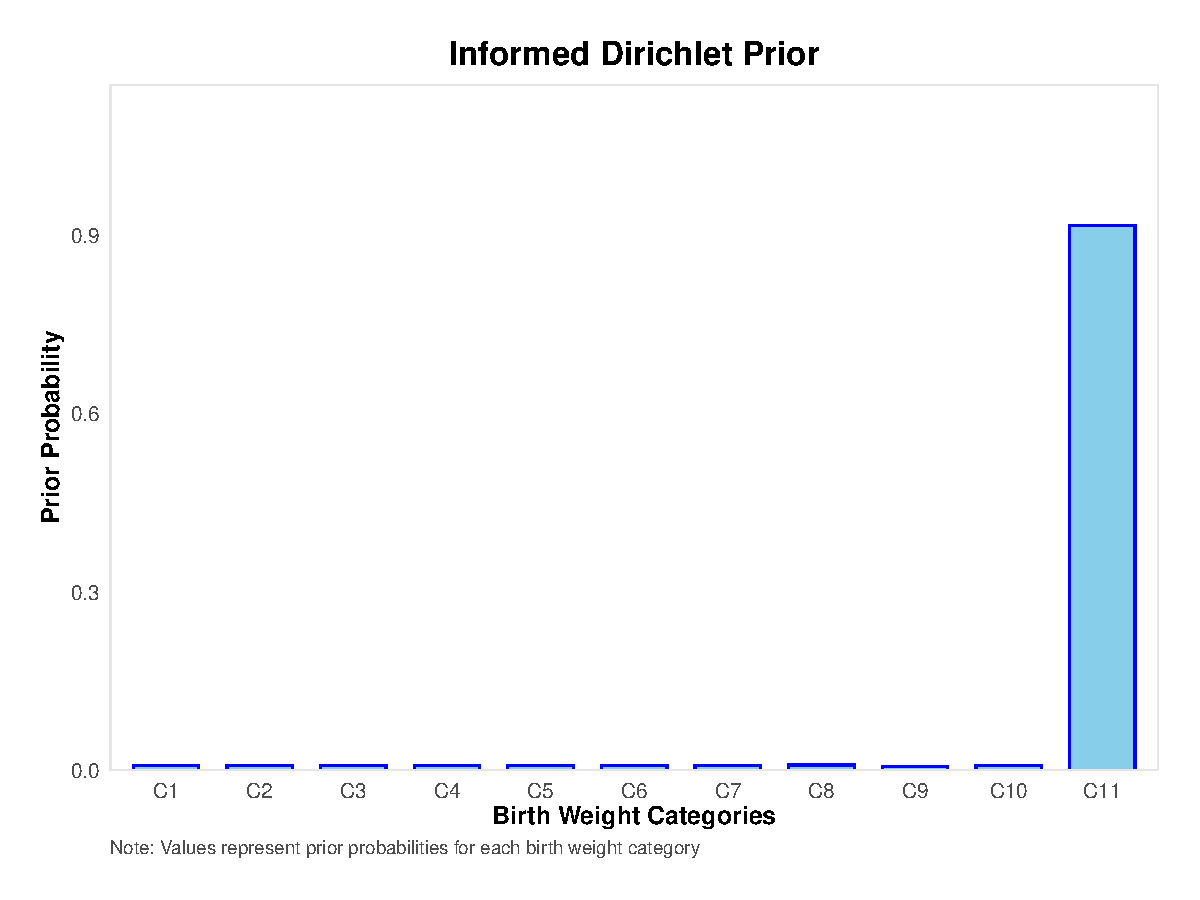
\includegraphics[width=6cm]{chapters/chapter3/figures/alphavec_plot_2020_full.pdf} }}
    \qquad
        \subfloat[\centering LBW-only model informed prior]{{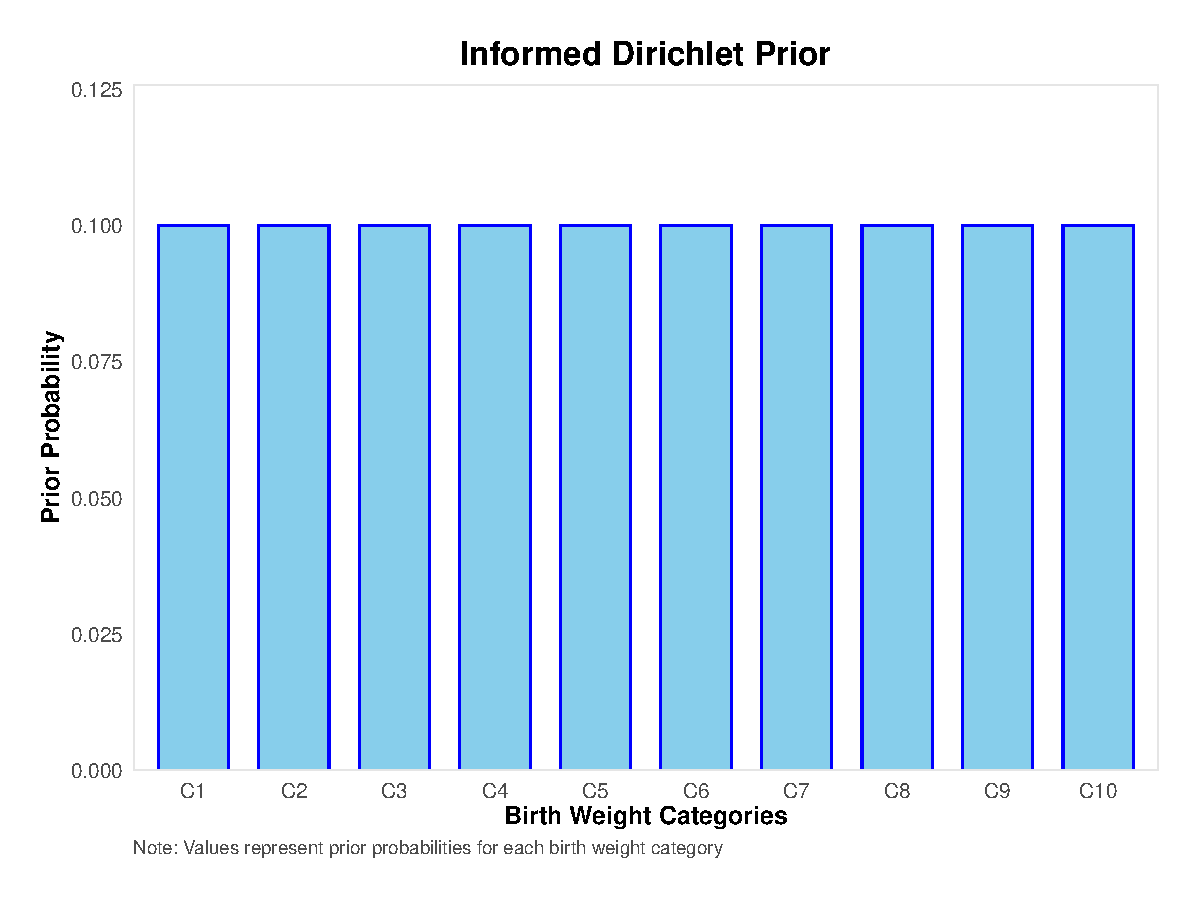
\includegraphics[width=6cm]{chapters/chapter3/figures/alphavec_plot_2020_small.pdf} }}
    \caption{Comparison of informed Dirichlet priors based on 2020 quantiles}
    \label{fig:alphavec}
\end{figure}


\section{DM-CART}
\label{sec:ch3-dm-cart}
\subsection{Custom Objective Function \& Splitting}
\label{sec:ch3-objective-function}
We fitted CART using \texttt{rpart}, in R \parencite{rpart_docs}, replacing the default Gini index with the adjusted marginal log DM likelihood or simply the log likelihood for brevity. Serving as our objective function, it output scores based on the reduction in deviance of a given split, i.e. negative log likelihood output \parencite{rpart_docs, intro_to_rpart}. When splitting, \texttt{rpart} computes the left and right split deviance calculation as in Section~\ref{sec:ch3-splits-in-cart}. For instance, suppose we propose a split on smoking status. The objective function evaluates separating the data into smoking and non-smoking mothers, as "distinct" on the count response vector. The improvement is the reduction in deviance, rewarding meaningful distributional shifts, thereby reducing heterogeneity in the node. Thus, distinctness here means the improvement gain from splitting under the predictor in question. Throughout, “risk’’ is used heuristically to describe a subpopulations relative prevalence of LBW outcomes.

\subsection{Tree Results and Insights: Full Model}
\label{sec:ch3-results}
For the full model, Figure~\ref{fig:tree} shows the hierarchical structure, and Figure~\ref{fig:full-model-ranked-imp} ranks improvement gain for each split. The full model splits as follows:

\begin{figure}[H]
  \centering
  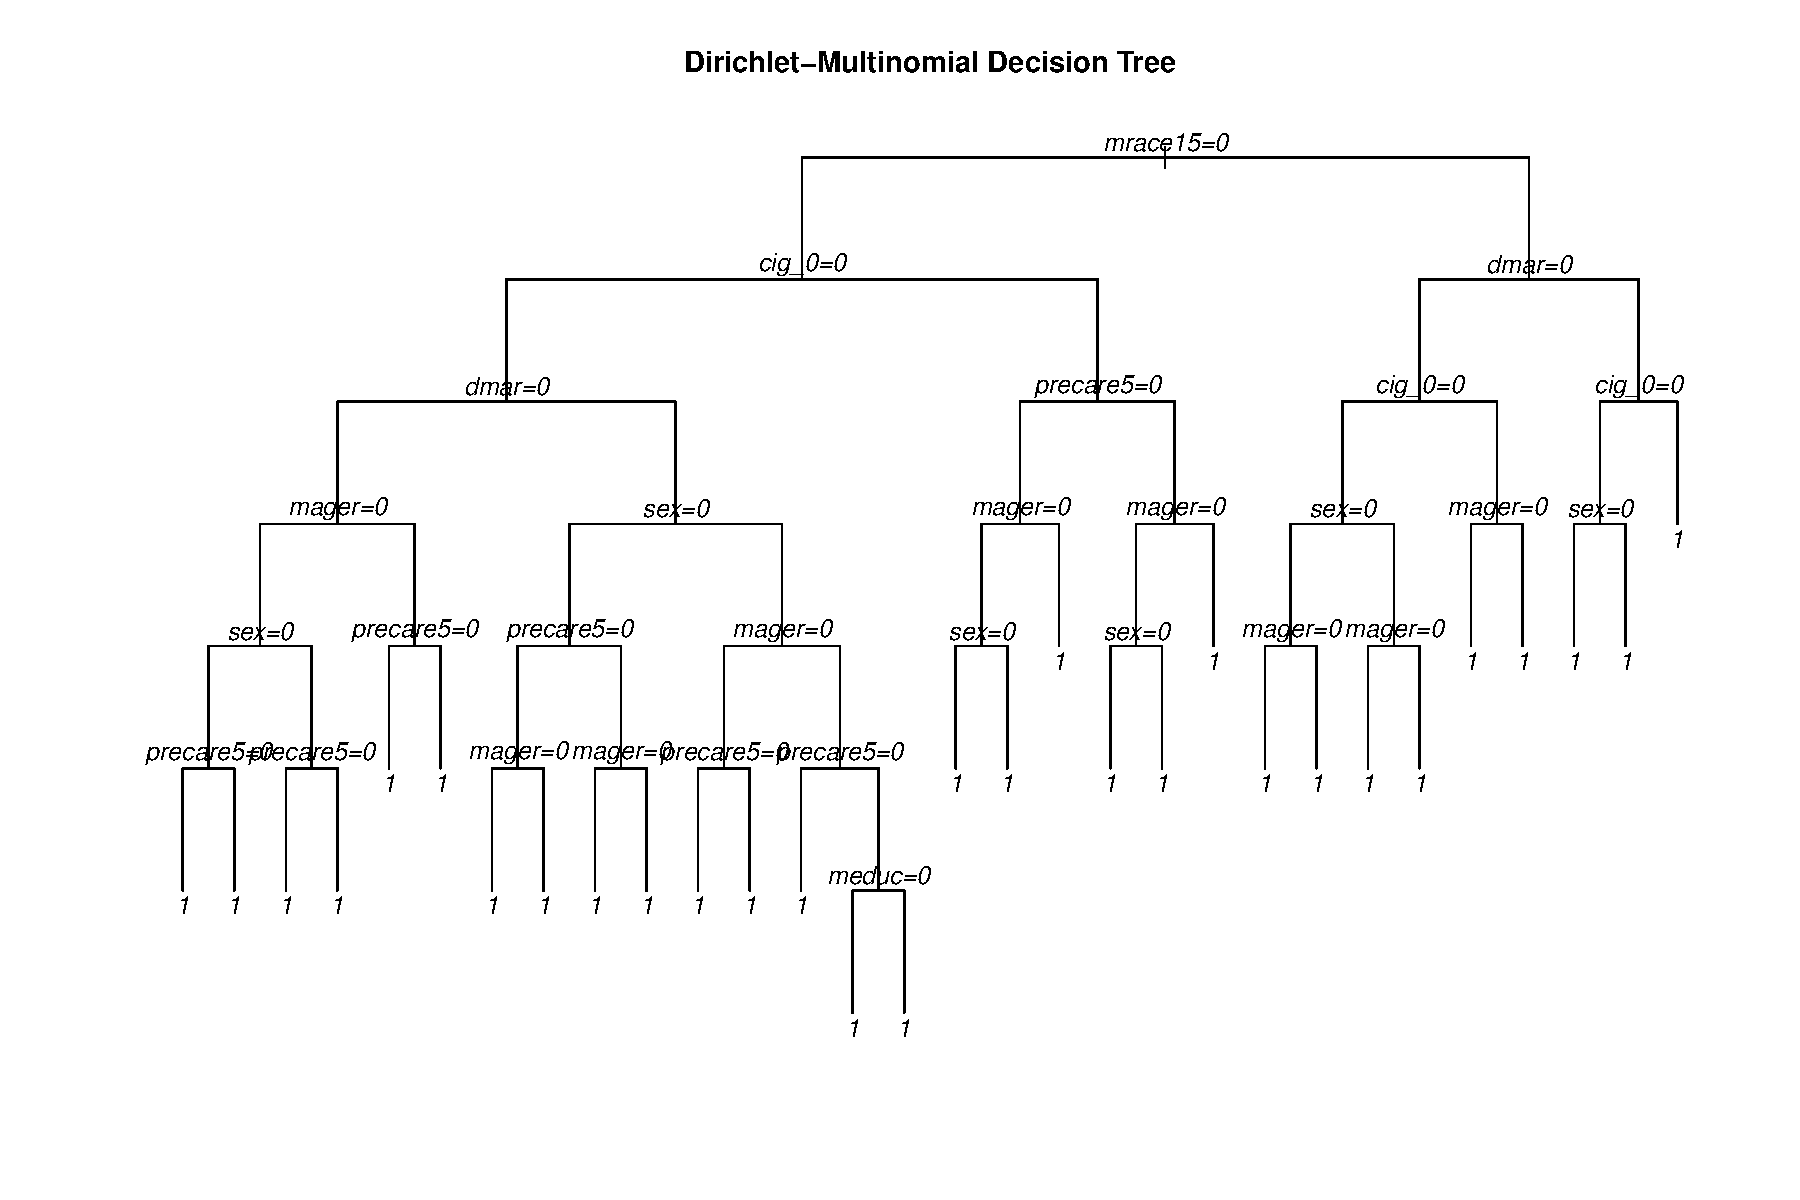
\includegraphics[width=1\textwidth]{chapters/chapter3/figures/dm_tree2021.pdf}
  \caption{Full model tree structure}
  \label{fig:tree}
\end{figure}

The root node contains all of the 2021 birth counts, and naturally the vast majority fall above 2.5 kg. The first, and largest deviance reduction, comes from separating the counts based on race, i.e. Black mothers (\texttt{mrace15}=1) from all other mothers (\texttt{mrace15}=0). This split yields the largest difference in birth-weight profiles and is shown to be the most informative predictor. This split aligns with documented discrepancies of race, playing a critical role in LBW incidence \parencite{kff_maternal_infant_health, pmc1751798}. Among Black mothers, smoking status supplies the next greatest improvement, whereas among non-Black mothers, smoking status is considered \emph{only after} marital status. That is to say, smoking most strongly differentiates outcomes for Black mothers, while partnership status matters more for non-Black mothers. These results show that further splits occur based on racial demographics. Further, analysis demonstrate that the overall highest risk subpopulations are among unmarried Black smokers, where \(\texttt{mrace15}=1,\texttt{cig\_0}=1, \texttt{dmar}=0\). Overall, race, smoking, and marital status jointly account for the bulk of the total improvement, confirming earlier evidence that Black smokers and unmarried non-Black mothers constitute the highest-risk subpopulations among racial demographics \parencite{kff_maternal_infant_health,pmc1751798, smoking_lbw} and Figure~\ref{fig:tree} and Figure~\ref{fig:full-model-ranked-imp} visualize these results. Further splitting down the branch of Black smokers provides further nuance of the highest-risk subgroups (\(\texttt{mrace15}=1,\texttt{cig\_0}=1, \texttt{dmar}=0\)). This node splits on infant gender, where on average, female infants weigh less than males \parencite{decreasing_sex_diff_birth_weight2009}. 

Generally, the lowest-risk subpopulations are where \texttt{mrace15}=0 — recall that smoking status is considered after marital status of the mother. Despite the ordering of ranked splits, smoking is a direct determinant of LBW incidence \parencite{smoking_lbw}. After socioeconomic and demographic variables are considered, the model emphasizes more biological and genetic predictors, namely gender, prenatal care, and maternal age. The lowest-risk groups where \(\texttt{mrace15}=0, \texttt{dmar}=1,\texttt{cig\_0}=0\), with age being the final predictor considered. Moreover, this branch has a depth of 4 while the highest-risk subgroups have a depth of 6 and 7. 

Surprisingly, the only case where education status (\texttt{meduc}) was used was when the mother was Black, non-smoker, below 33 years old, without adequate prenatal care, and had a female newborn, (i.e. \(\texttt{mrace15} = 1, \texttt{cig\_0} = 0,\texttt{dmar}=0, \texttt{sex}=0, \texttt{mager}=0,\texttt{precare5}=0\)). Given that education has been noted by many \parencite{edu_lbw} to have an effect on socioeconomic conditions, namely earnings, which might not be as strong of a predictor as initially thought.

The full model structure provides insights into the direct risk stratification. This approach finds race, smoking status, and marital status as the dominant predictors, ranked as the top three splits in Figure~\ref{fig:full-model-ranked-imp}. The model shifts then toward biological predictors of maternal age, infant gender, and adequacy of prenatal care. Lastly education status is only used in one split, providing the least improvement. 

\subsection{Tree Results and Insights: LBW-Only}
\label{sec:ch3-comparison}

\begin{figure}[H]
  \centering
  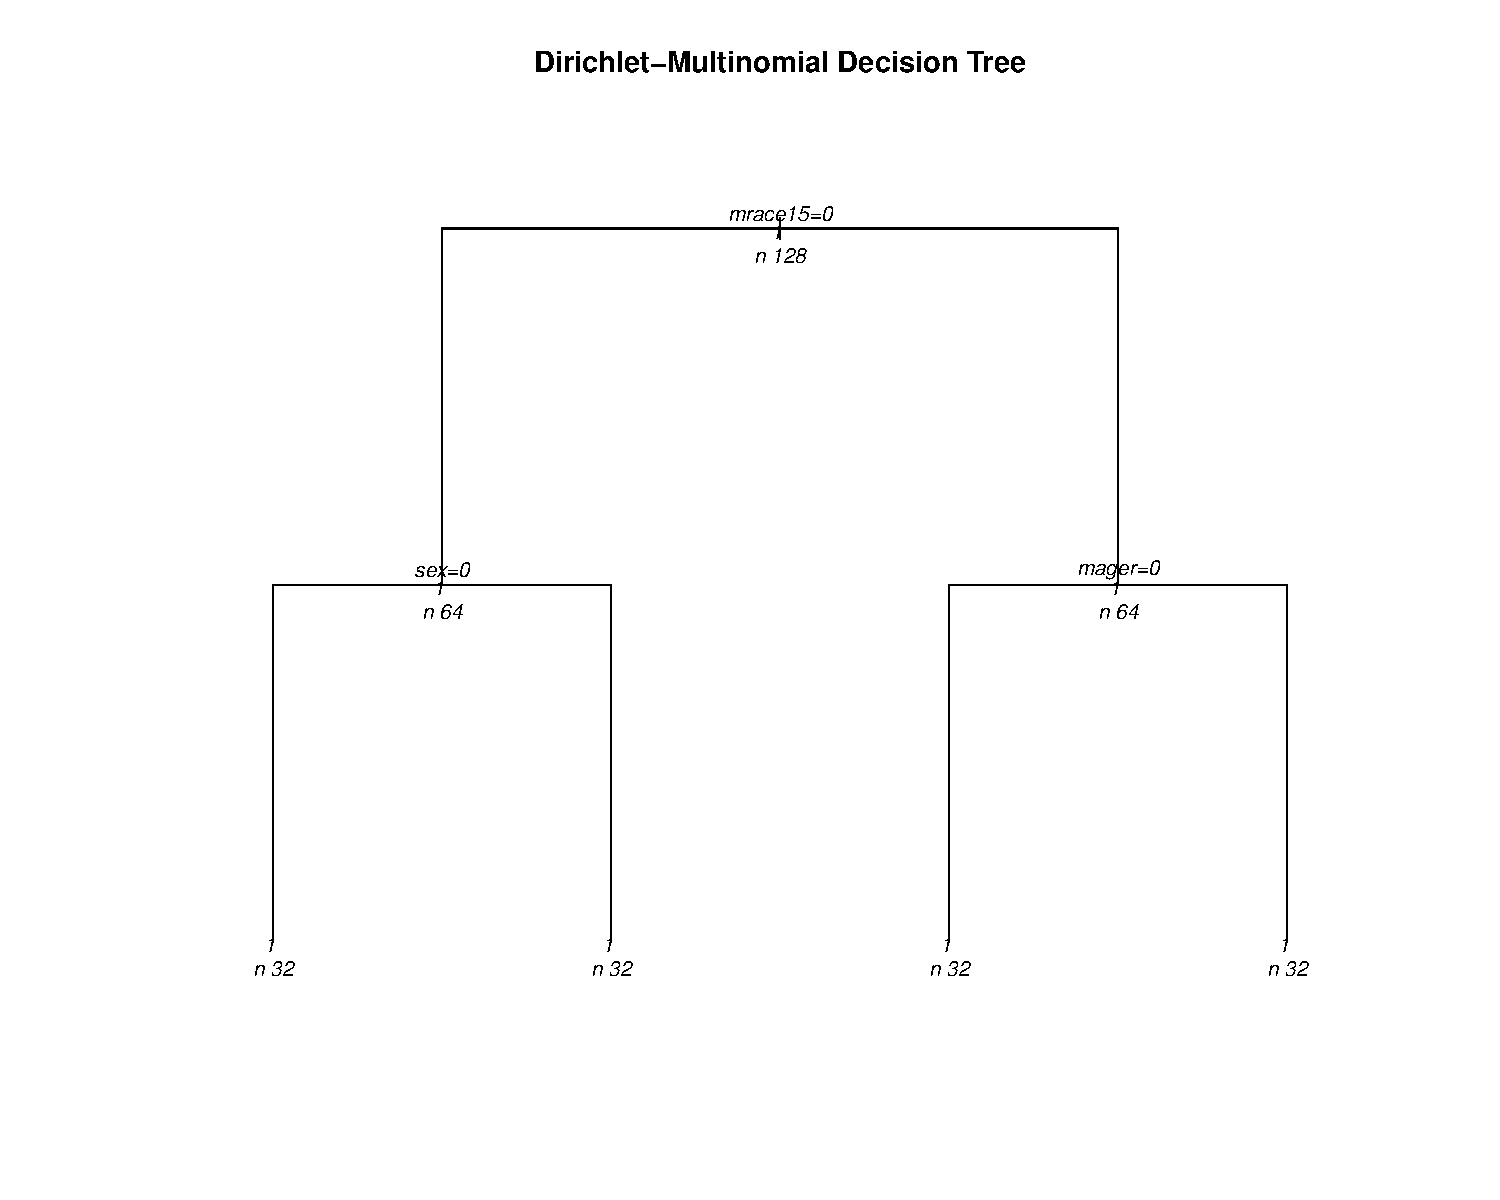
\includegraphics[width=1\textwidth]{chapters/chapter3/figures/dm_tree2021_2.pdf}
  \caption{LBW-only model tree structure}
  \label{fig:tree_2}
\end{figure}

As seen in Figure~\ref{fig:tree_2}, the restriction to only LBW observations drastically changes the tree's structure. The distributional contrast between NBW and LBW disappears by this restriction. Initially, this model has more homogeneity in the data yielding less drastic improvements. Race again dominates the root split, with the second-level splitters being now infant gender for the \texttt{mrace15}=1 branch, and maternal age for the \texttt{mrace15}=0 branch; with smoking status, and marital status \emph{never} appearing. By every infant already being below 2.5 kg., behavioral and socioeconomic factors that distinguish NBW and LBW, no longer provide useful partitions. Instead, biological factors explain within-LBW heterogeneity. A key takeaway from contrasting the two models is that the LBW-only model suggests Black mothers \textit{continue} to have a higher incidence of LBW newborns. 

Variable importance among the full and LBW-only model are drastically different as well. Figures~\ref{fig:full-model-ranked-imp} and \ref{fig:lbw-model-ranked-imp} order predictors by the sum of total deviance each eliminates across all splits, showing the contrast between predictor usage. The barplots reflects the greedy search of CART, where early splits absorb a large share of heterogeneity and later splits improve the fit only marginally, regardless of their actual effect on the response \parencite{cart_greedy}.   

\subsection{Depth-Controlled Model Comparison}
\label{sec:ch3-comparison-depth}

To investigate how different models select variables as the tree grows, we refit both the full and LBW-only CART models at maximum depths of 2, 3, 4, 5, while explicitly tracking the smoking predictor to discern its roles among other predictors in different modeling contexts. Figures~\ref{fig:trees-comparison-full} and~\ref{fig:trees-comparison-lbw} visualize the trees.

As the depths increase for the full model (Figure~\ref{fig:trees-comparison-full}), the number of terminal nodes expands from 4 at depths 2, to 19 at depth of 5, while the number of predictors rises from 3 to 6. Race, infant gender, and marital status appear in every depth while maternal age and prenatal care are included at depth 4. Moreover,  \texttt{cig\_0} is selected at only at depths 4 and 5, suggesting that once additional socioeconomic and biological variables are available, smoking contributes little deviance reduction with the full spectrum of birth-weight outcomes. 

The LBW-restricted trees (Figure~\ref{fig:trees-comparison-lbw}) the growth complexity stagnates after depth of 3, starting at 4 terminal nodes at depth of 2 growing to only 5 at depth 3 through 5. The lessened number of leaves reflects the large homogeneity in the restricted LBW data. Like the full model, the initial splitter is race and subsequent splits consider infant gender, maternal age, then considering prenatal care adequacy \emph{only for Black male newborns} (\(\texttt{mrace15} = 1, \texttt{sex}=1\)). These results highlight the stark contrast between the full model's ending complexity. Here, we consider how race, maternal age, infant gender, and prenatal care effect LBW severity among LBW cases. Crucially, the predictors of \texttt{cig\_0}, \texttt{dmar}, and \texttt{meduc} are never considered, demonstrating that such socioeconomic factors do not play a critical role in identifying added risk among LBW outcomes. That is to say that, smoking, marital status, and educational attainment do not significantly contribute to increased LBW severity.

It is clear that the predictor hierarchy and prioritization has shifted when the depth parameter is restricted compared to the first fit LBW-only model in Section~\ref{sec:ch3-comparison}. Due to this difference, we will employ a two-tier bootstrap procedure to confirm stability of variable selection and importance. 

% depth comparison - FULL
\begin{figure}[p]
    \centering
    % First row
    \begin{minipage}{0.48\textwidth}
        \centering
        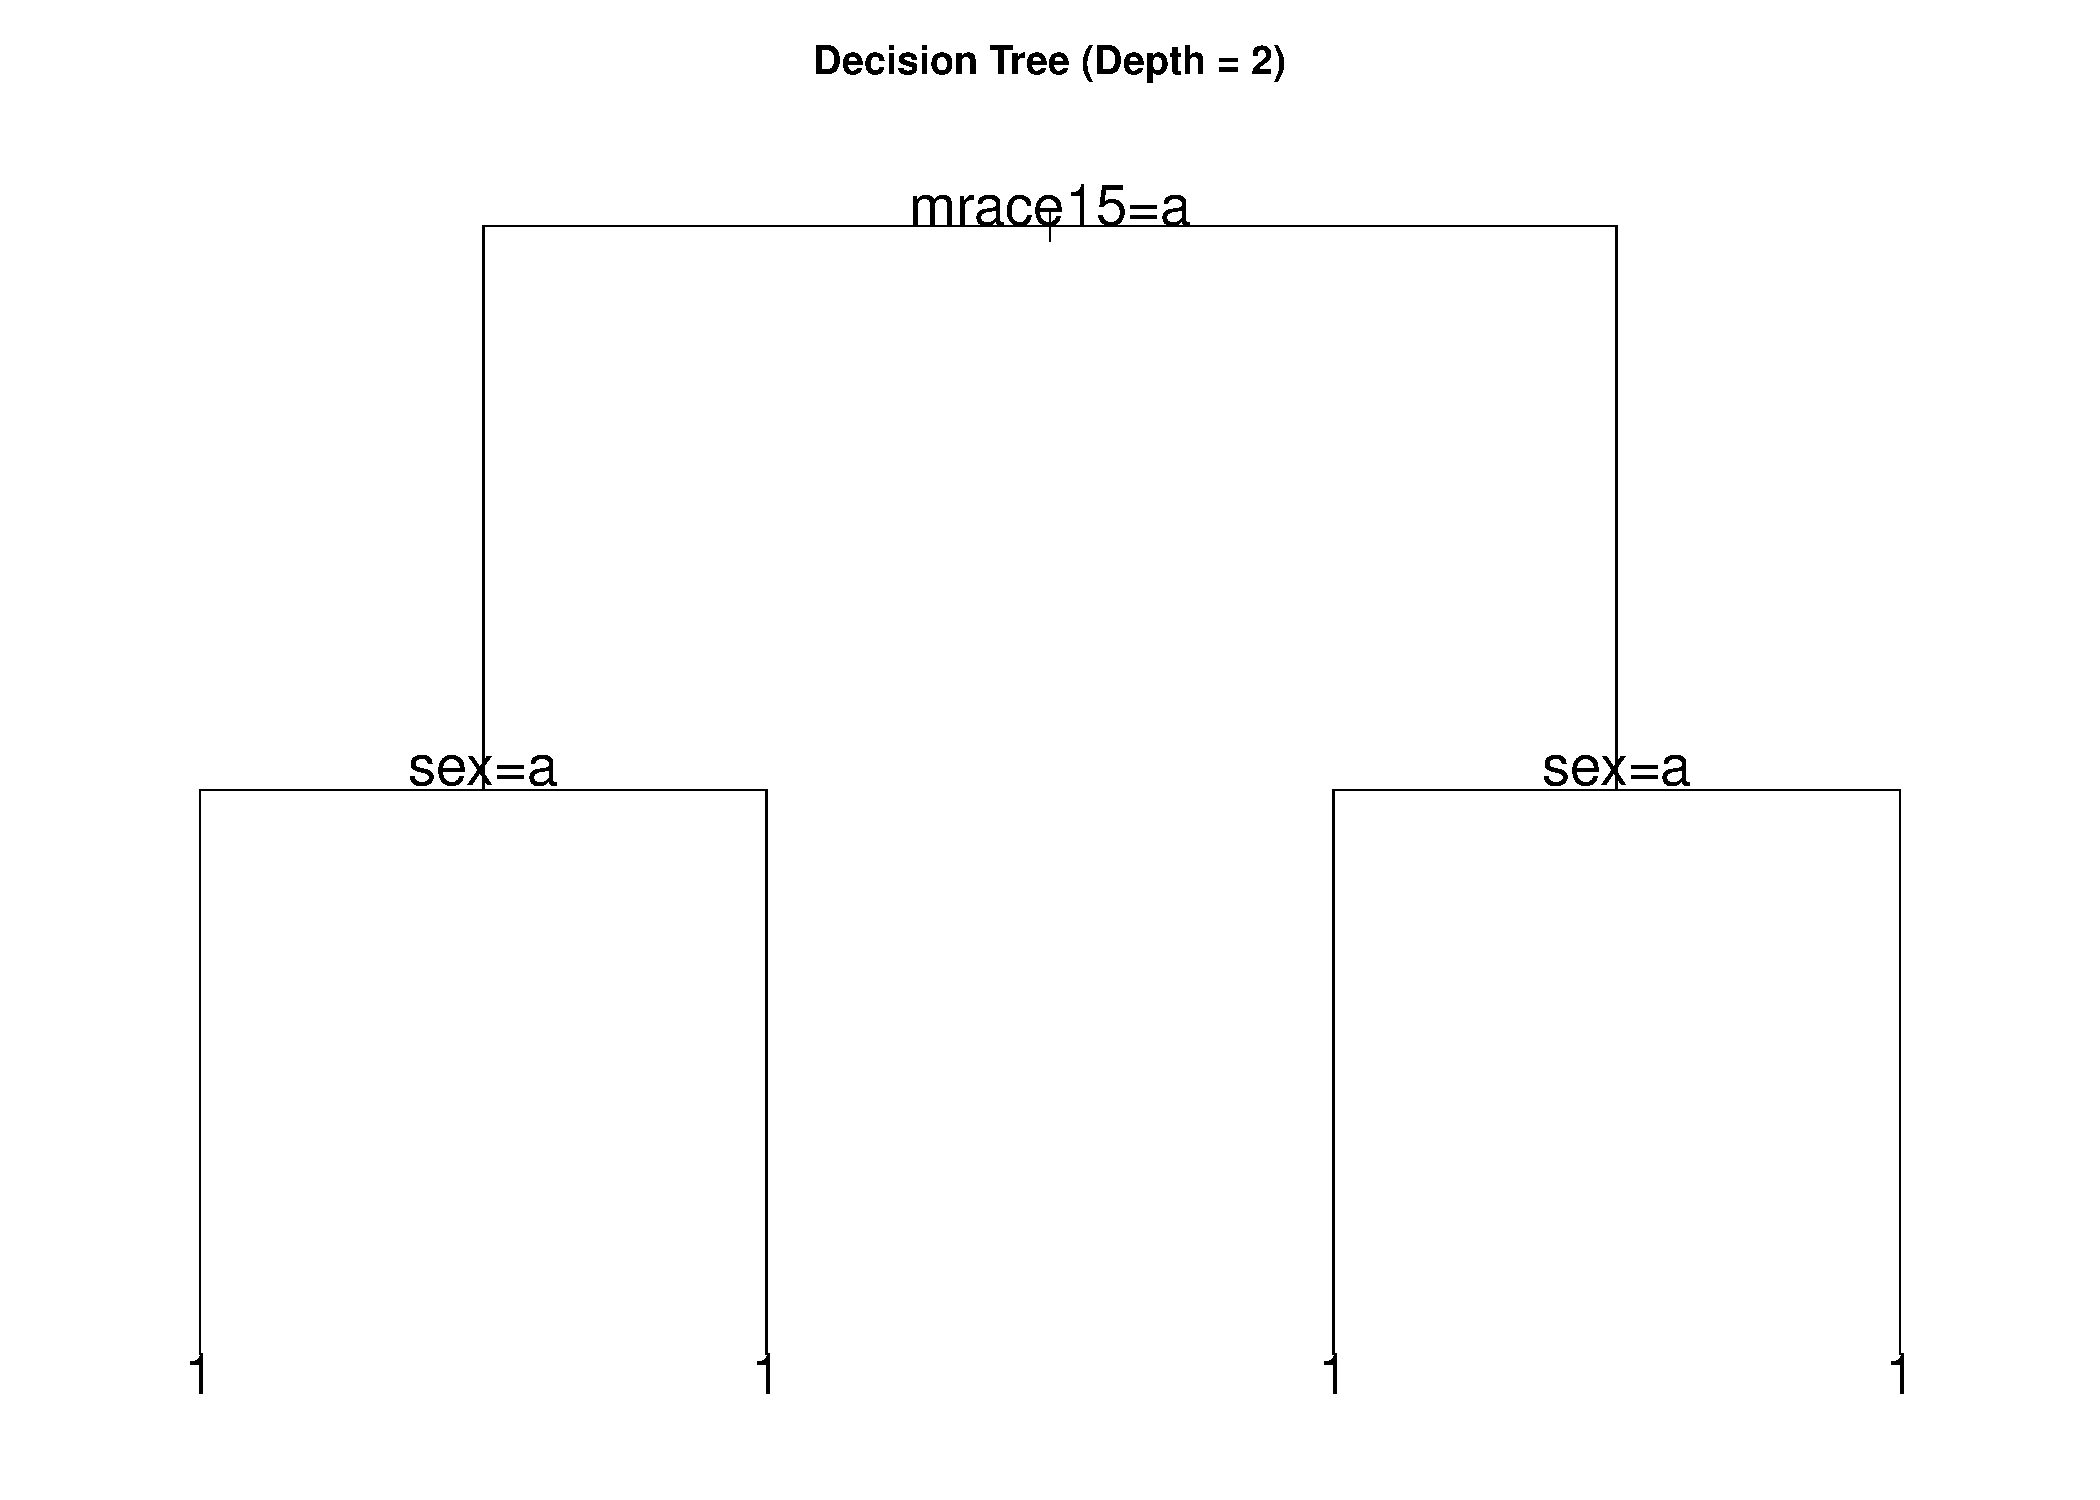
\includegraphics[width=\linewidth]{chapters/chapter3/figures/depth/plot1/decision_tree_depth_2_2021_large.pdf}
        \caption*{Maximum depth = 2}
    \end{minipage}
    \hspace{0.02\textwidth}
    \begin{minipage}{0.48\textwidth}
        \centering
        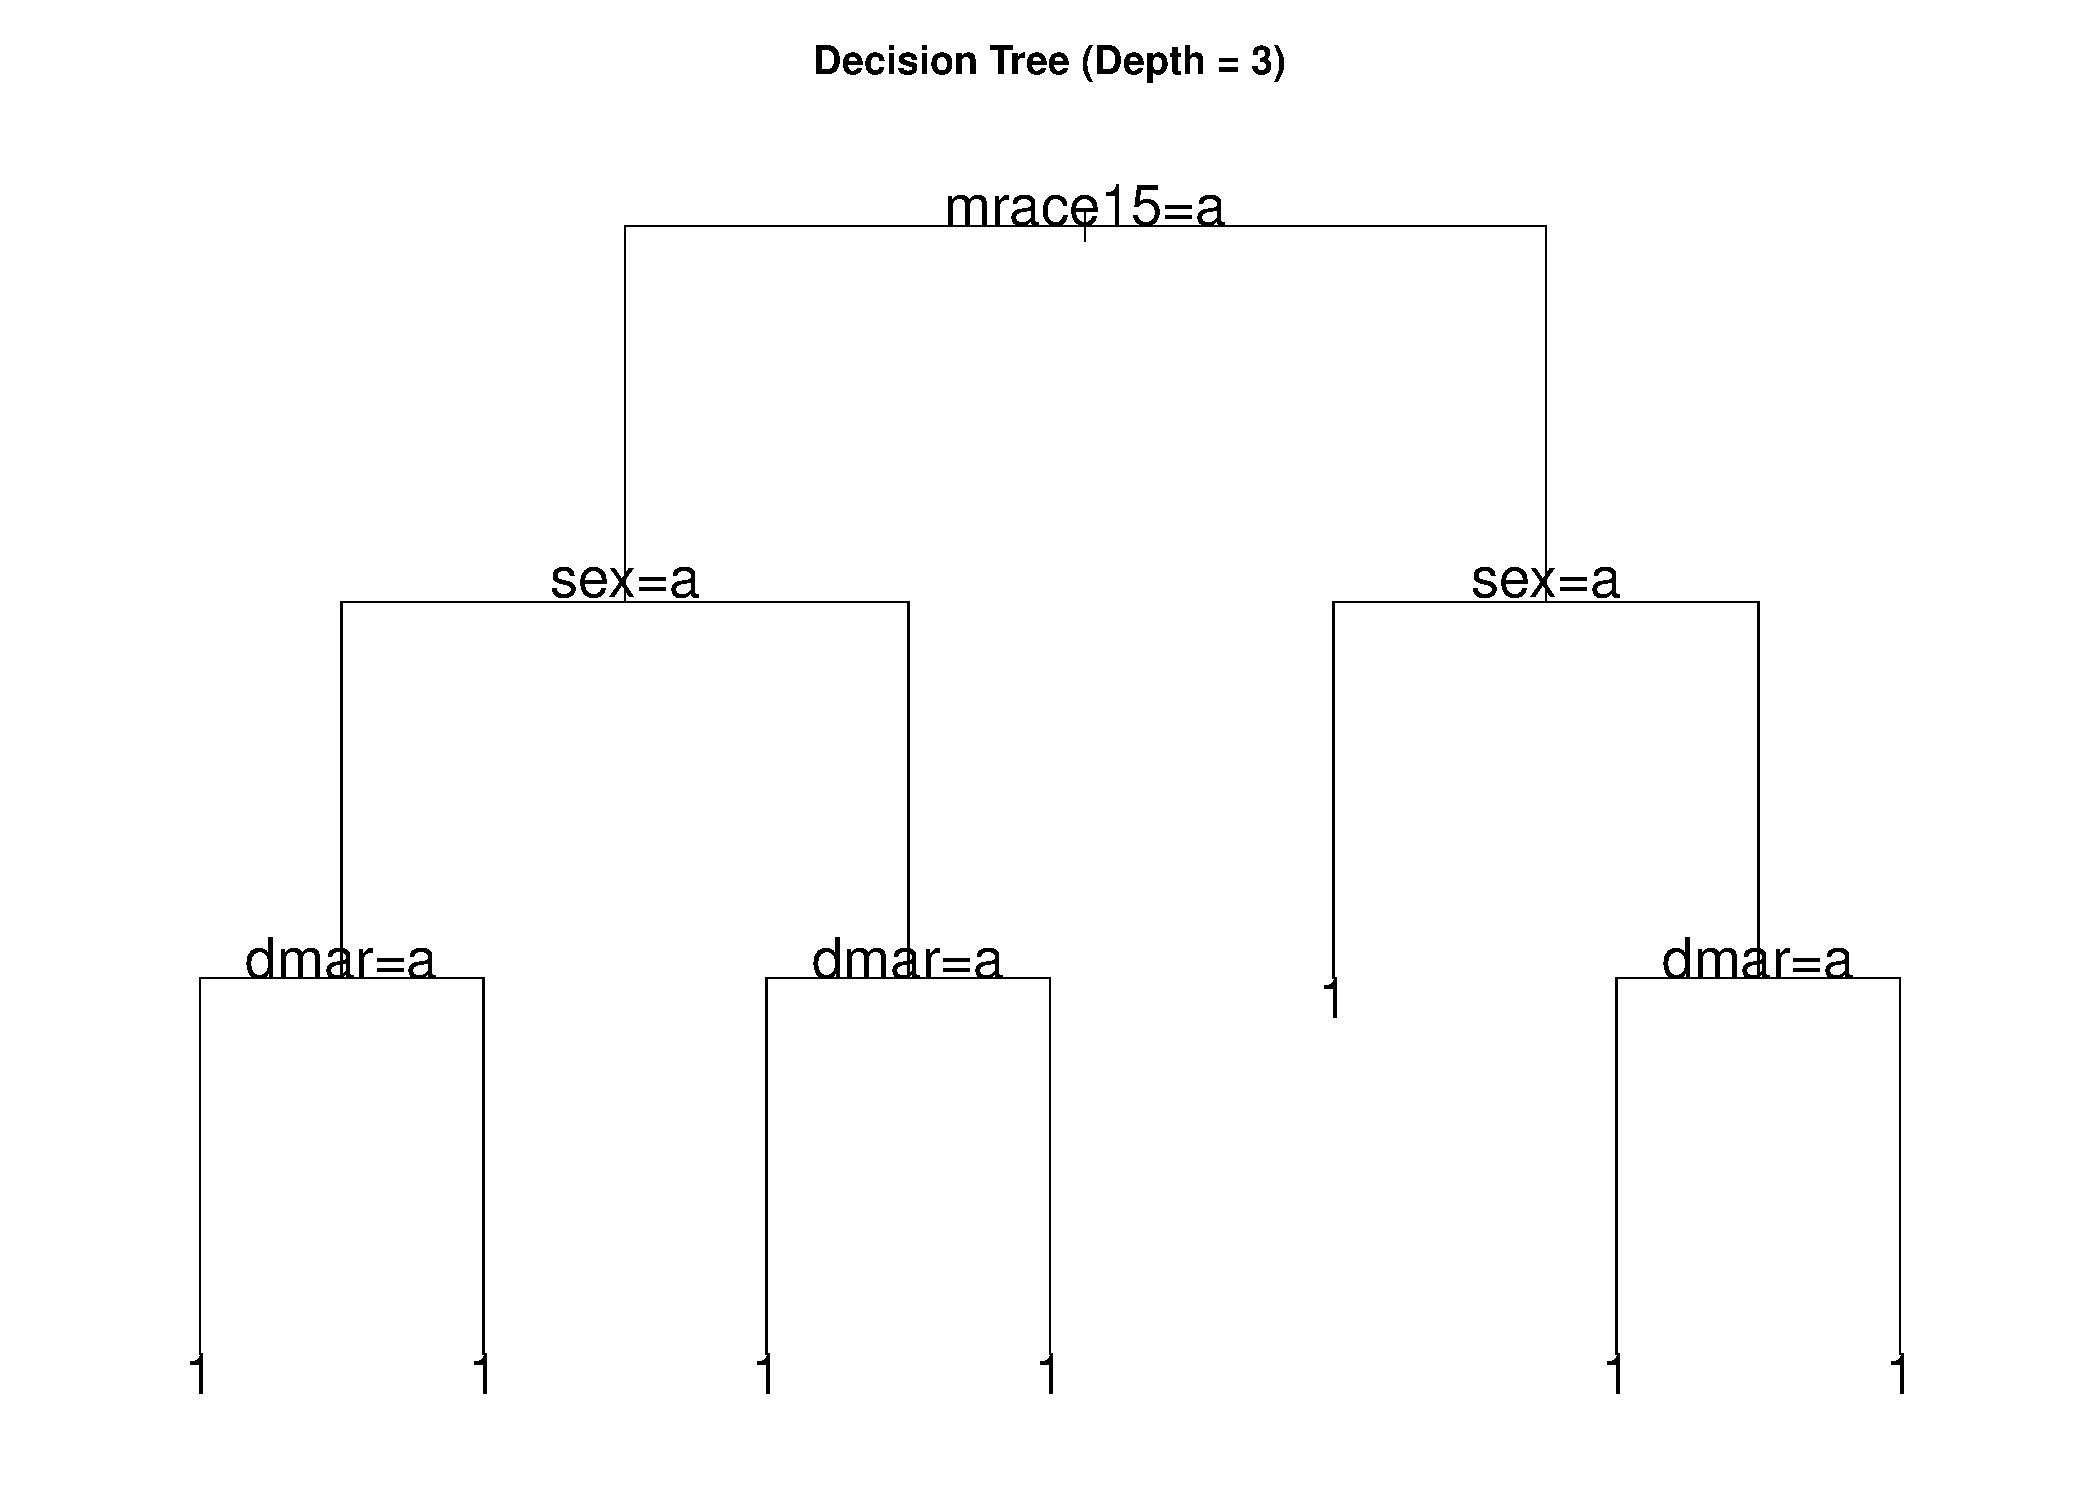
\includegraphics[width=\linewidth]{chapters/chapter3/figures/depth/plot1/decision_tree_depth_3_2021_large.pdf}
        \caption*{Maximum depth = 3}
    \end{minipage}
    
    \vspace{1cm}
    
    % Second row
    \begin{minipage}{0.48\textwidth}
        \centering
        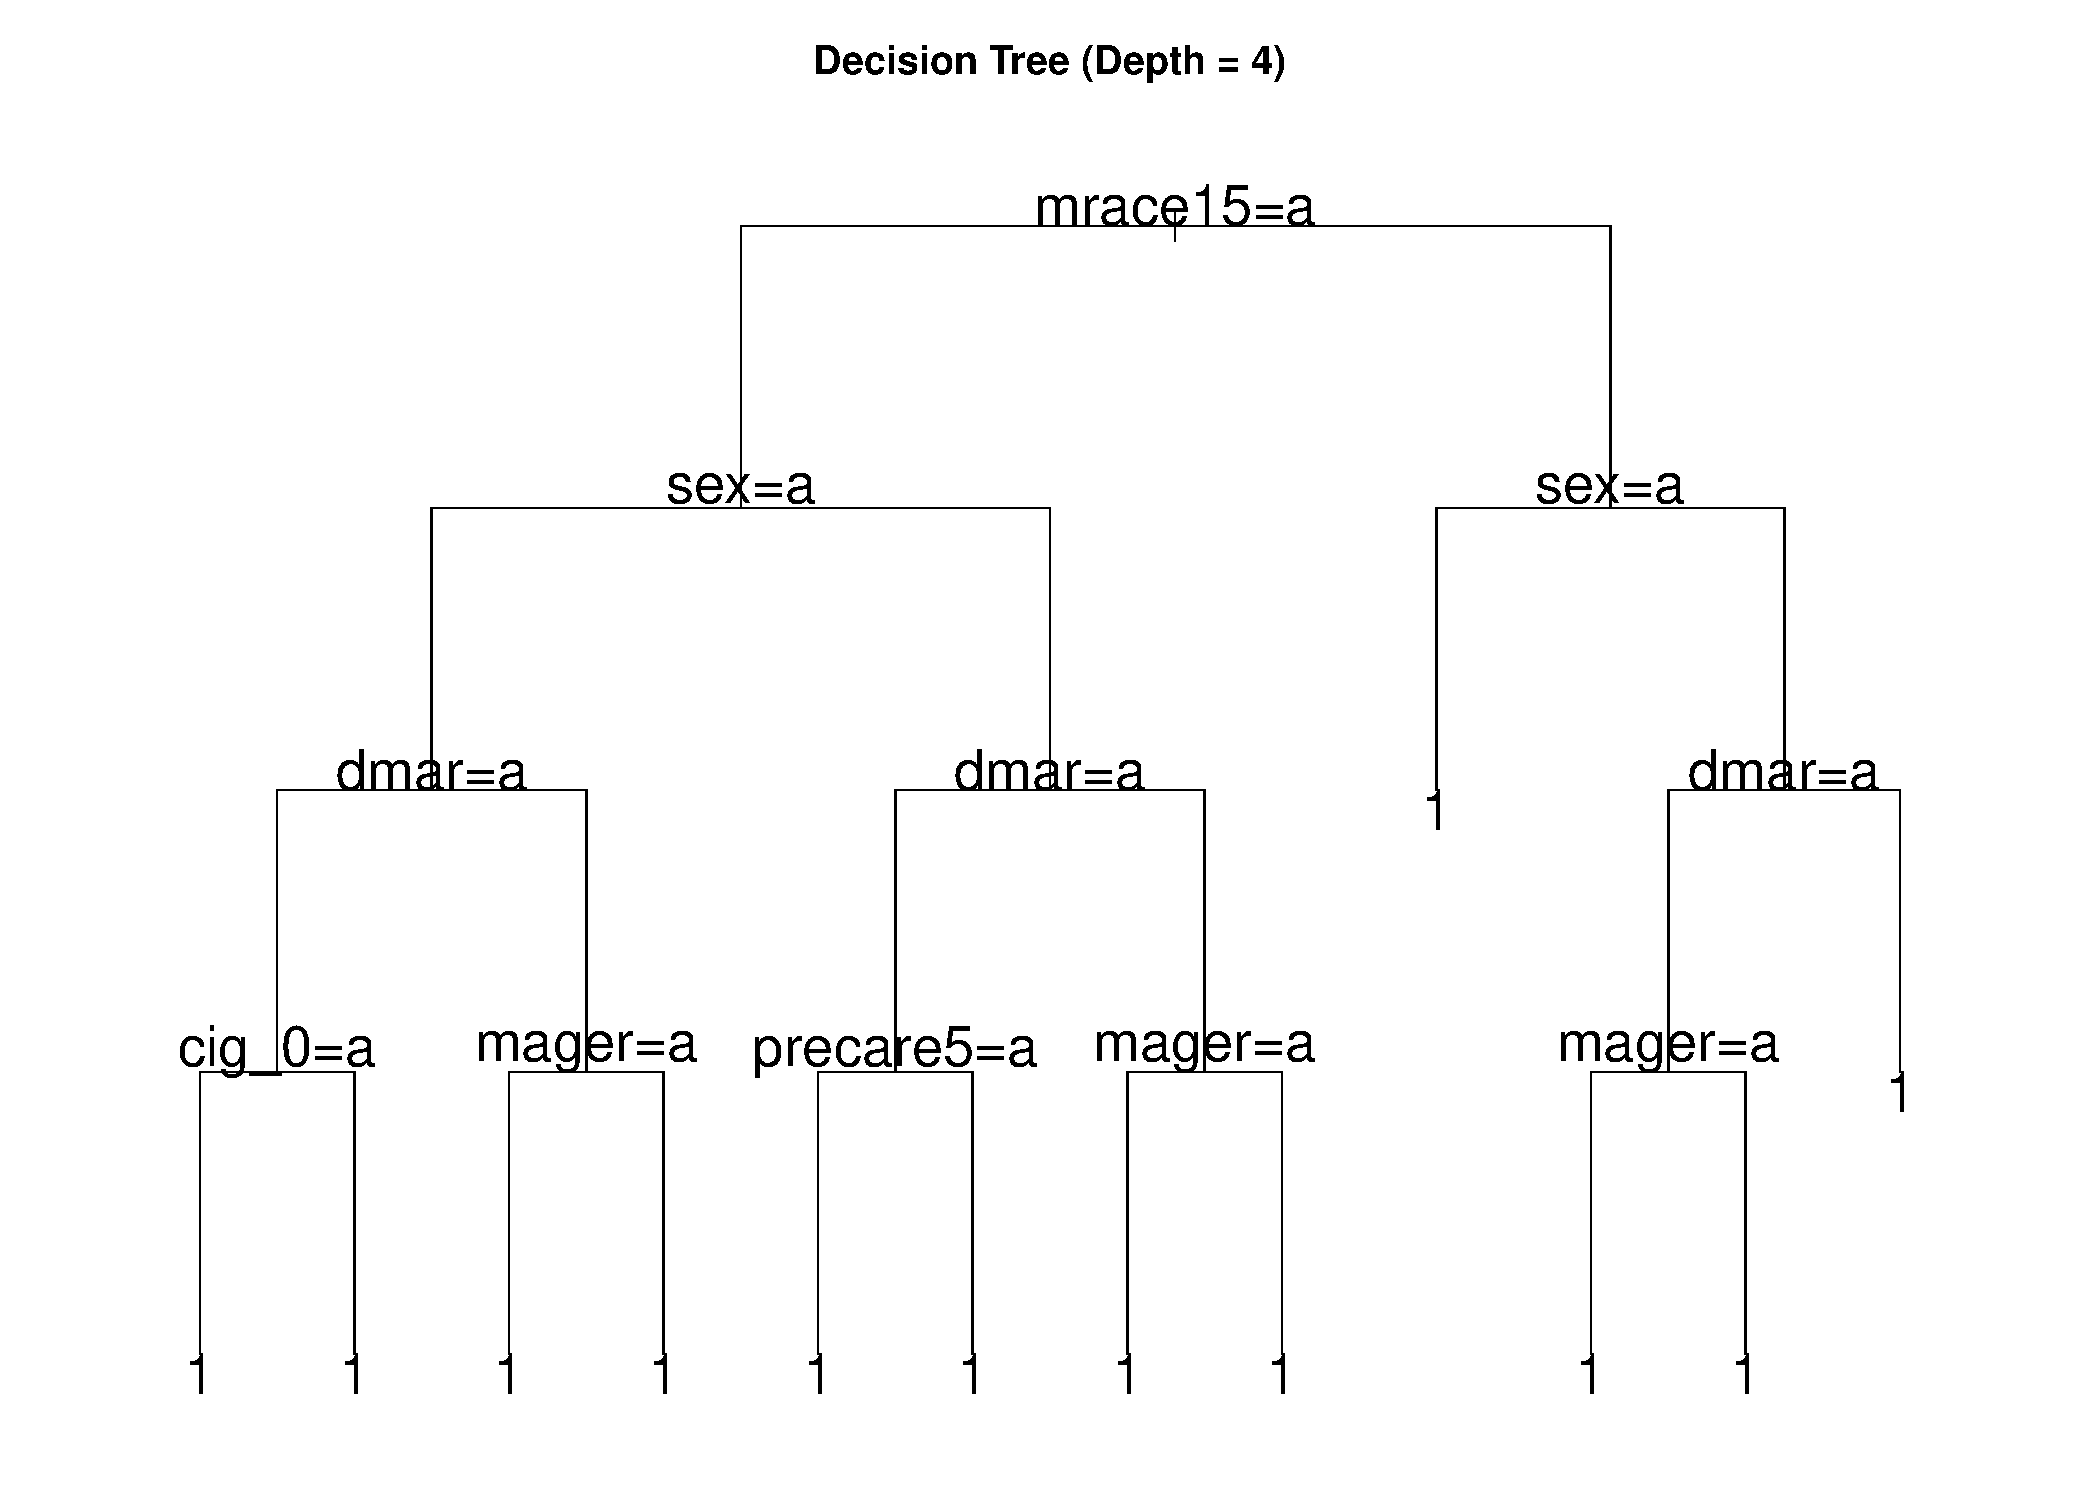
\includegraphics[width=\linewidth]{chapters/chapter3/figures/depth/plot1/decision_tree_depth_4_2021_large.pdf}
        \caption*{Maximum depth = 4}
    \end{minipage}
    \hspace{0.02\textwidth}
    \begin{minipage}{0.48\textwidth}
        \centering
        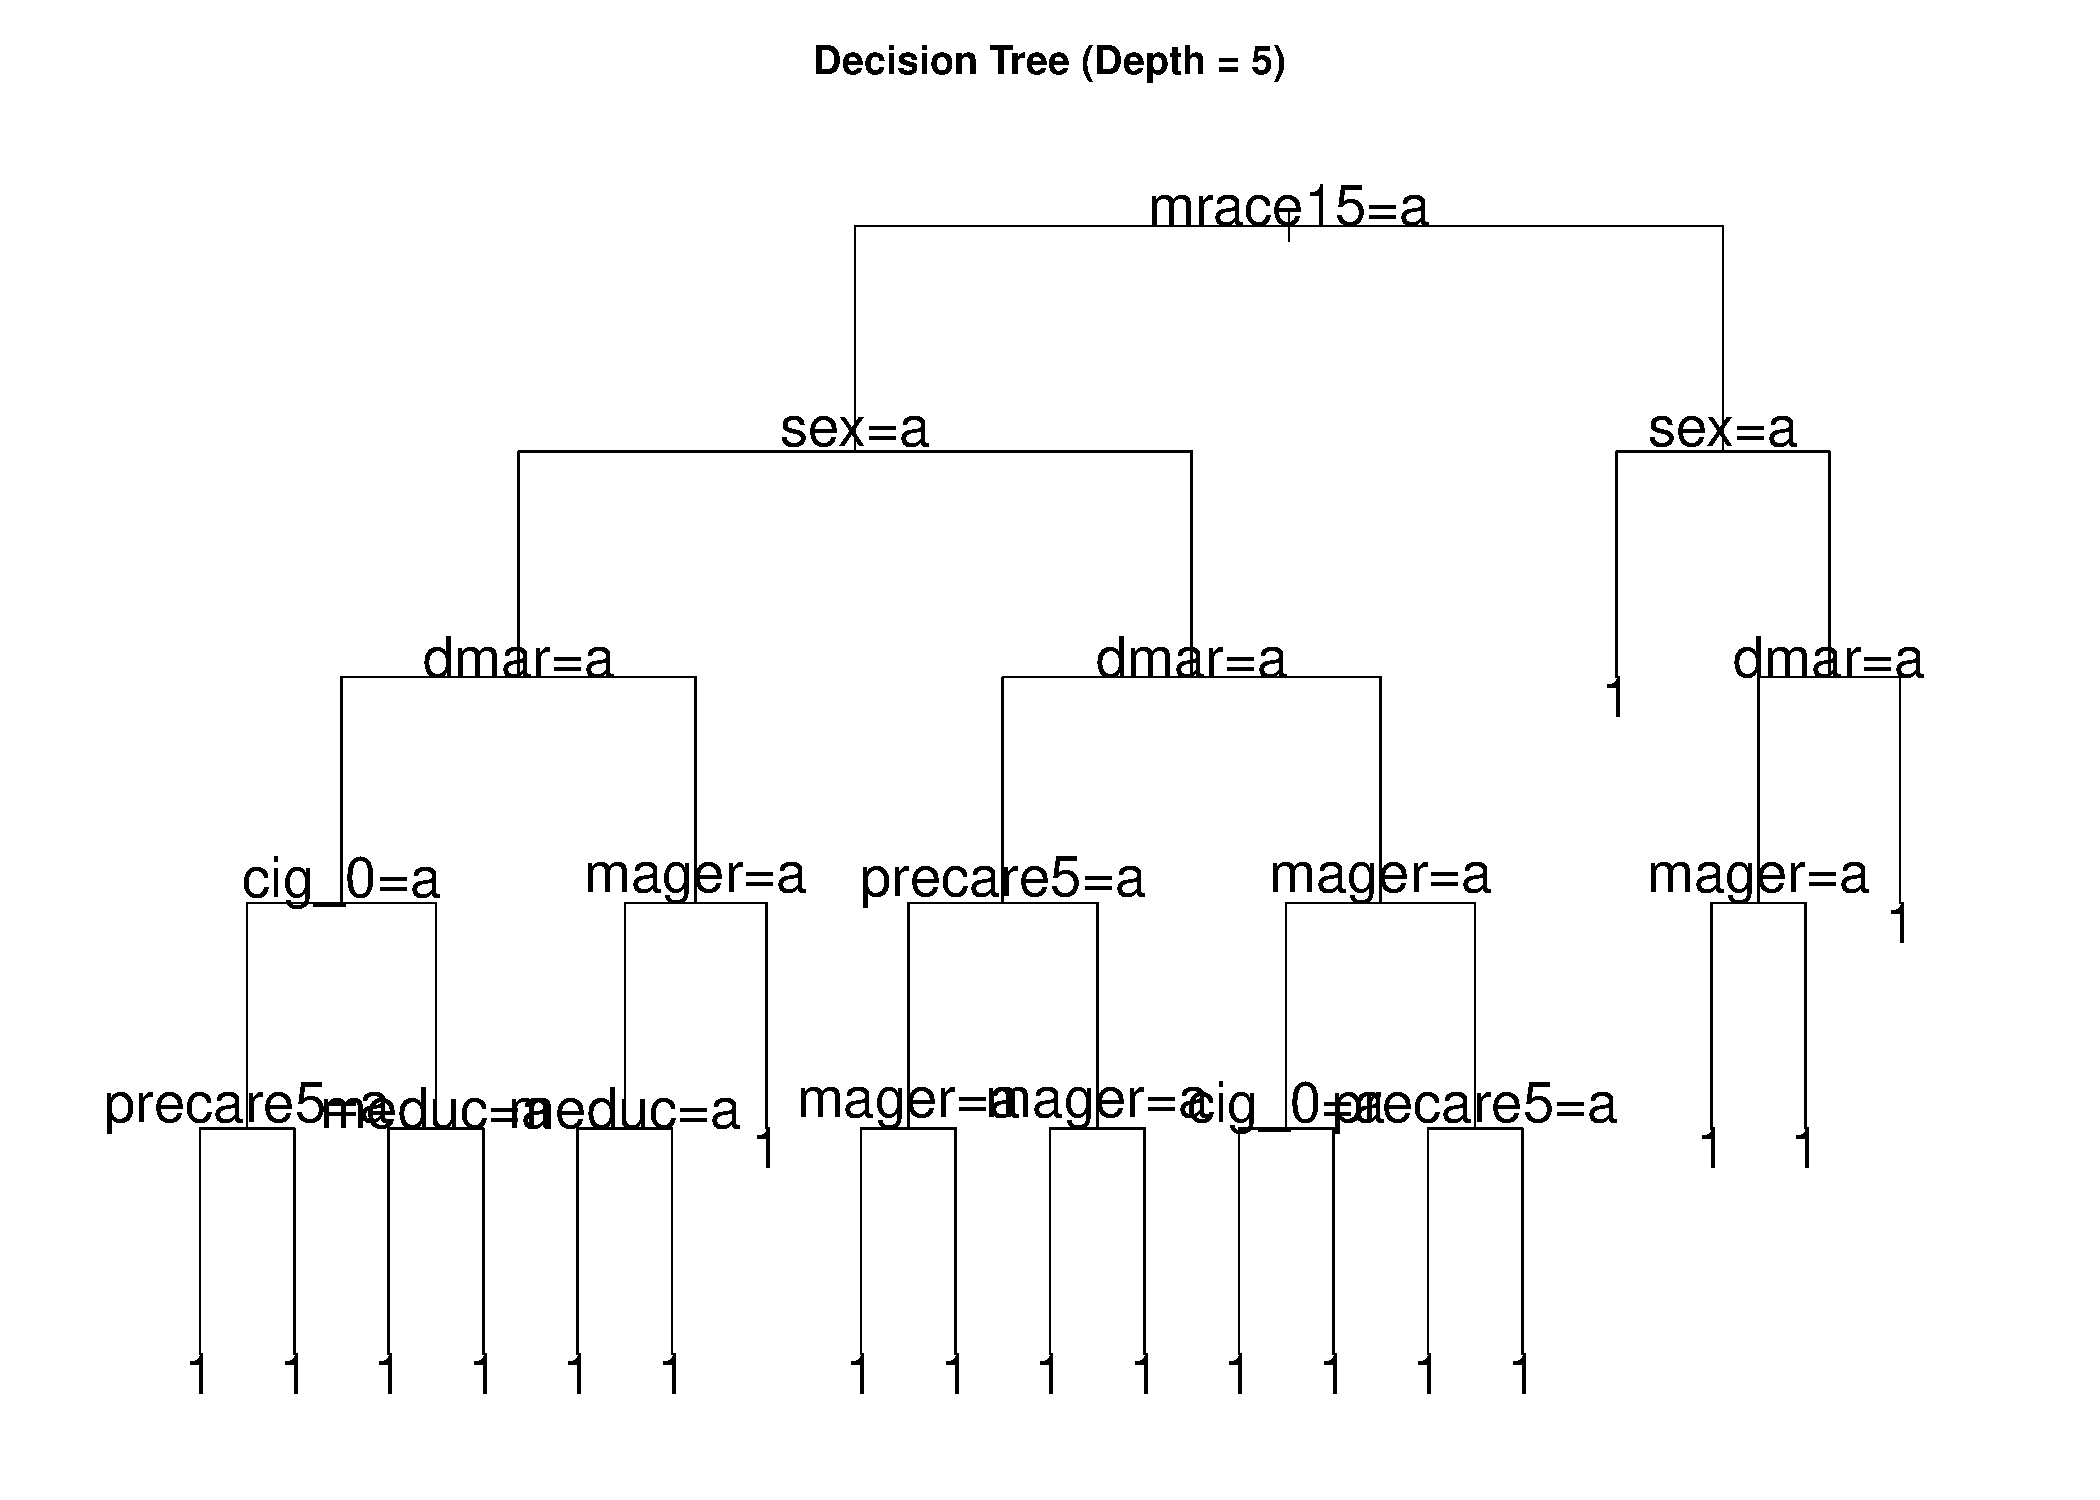
\includegraphics[width=\linewidth]{chapters/chapter3/figures/depth/plot1/decision_tree_depth_5_2021_large.pdf}
        \caption*{Maximum depth = 5}
    \end{minipage}
    \caption{Full model tree structures, showing growth patterns at different maximum depths (2,3,4,5). The trees demonstrate variable selection patterns with increasing depth, highlighting the growing complexity of the model structure.}
    \label{fig:trees-comparison-full}
\end{figure}

% depth comparison - LBW
\begin{figure}[p]
    \centering
    % First row
    \begin{minipage}{0.48\textwidth}
        \centering
        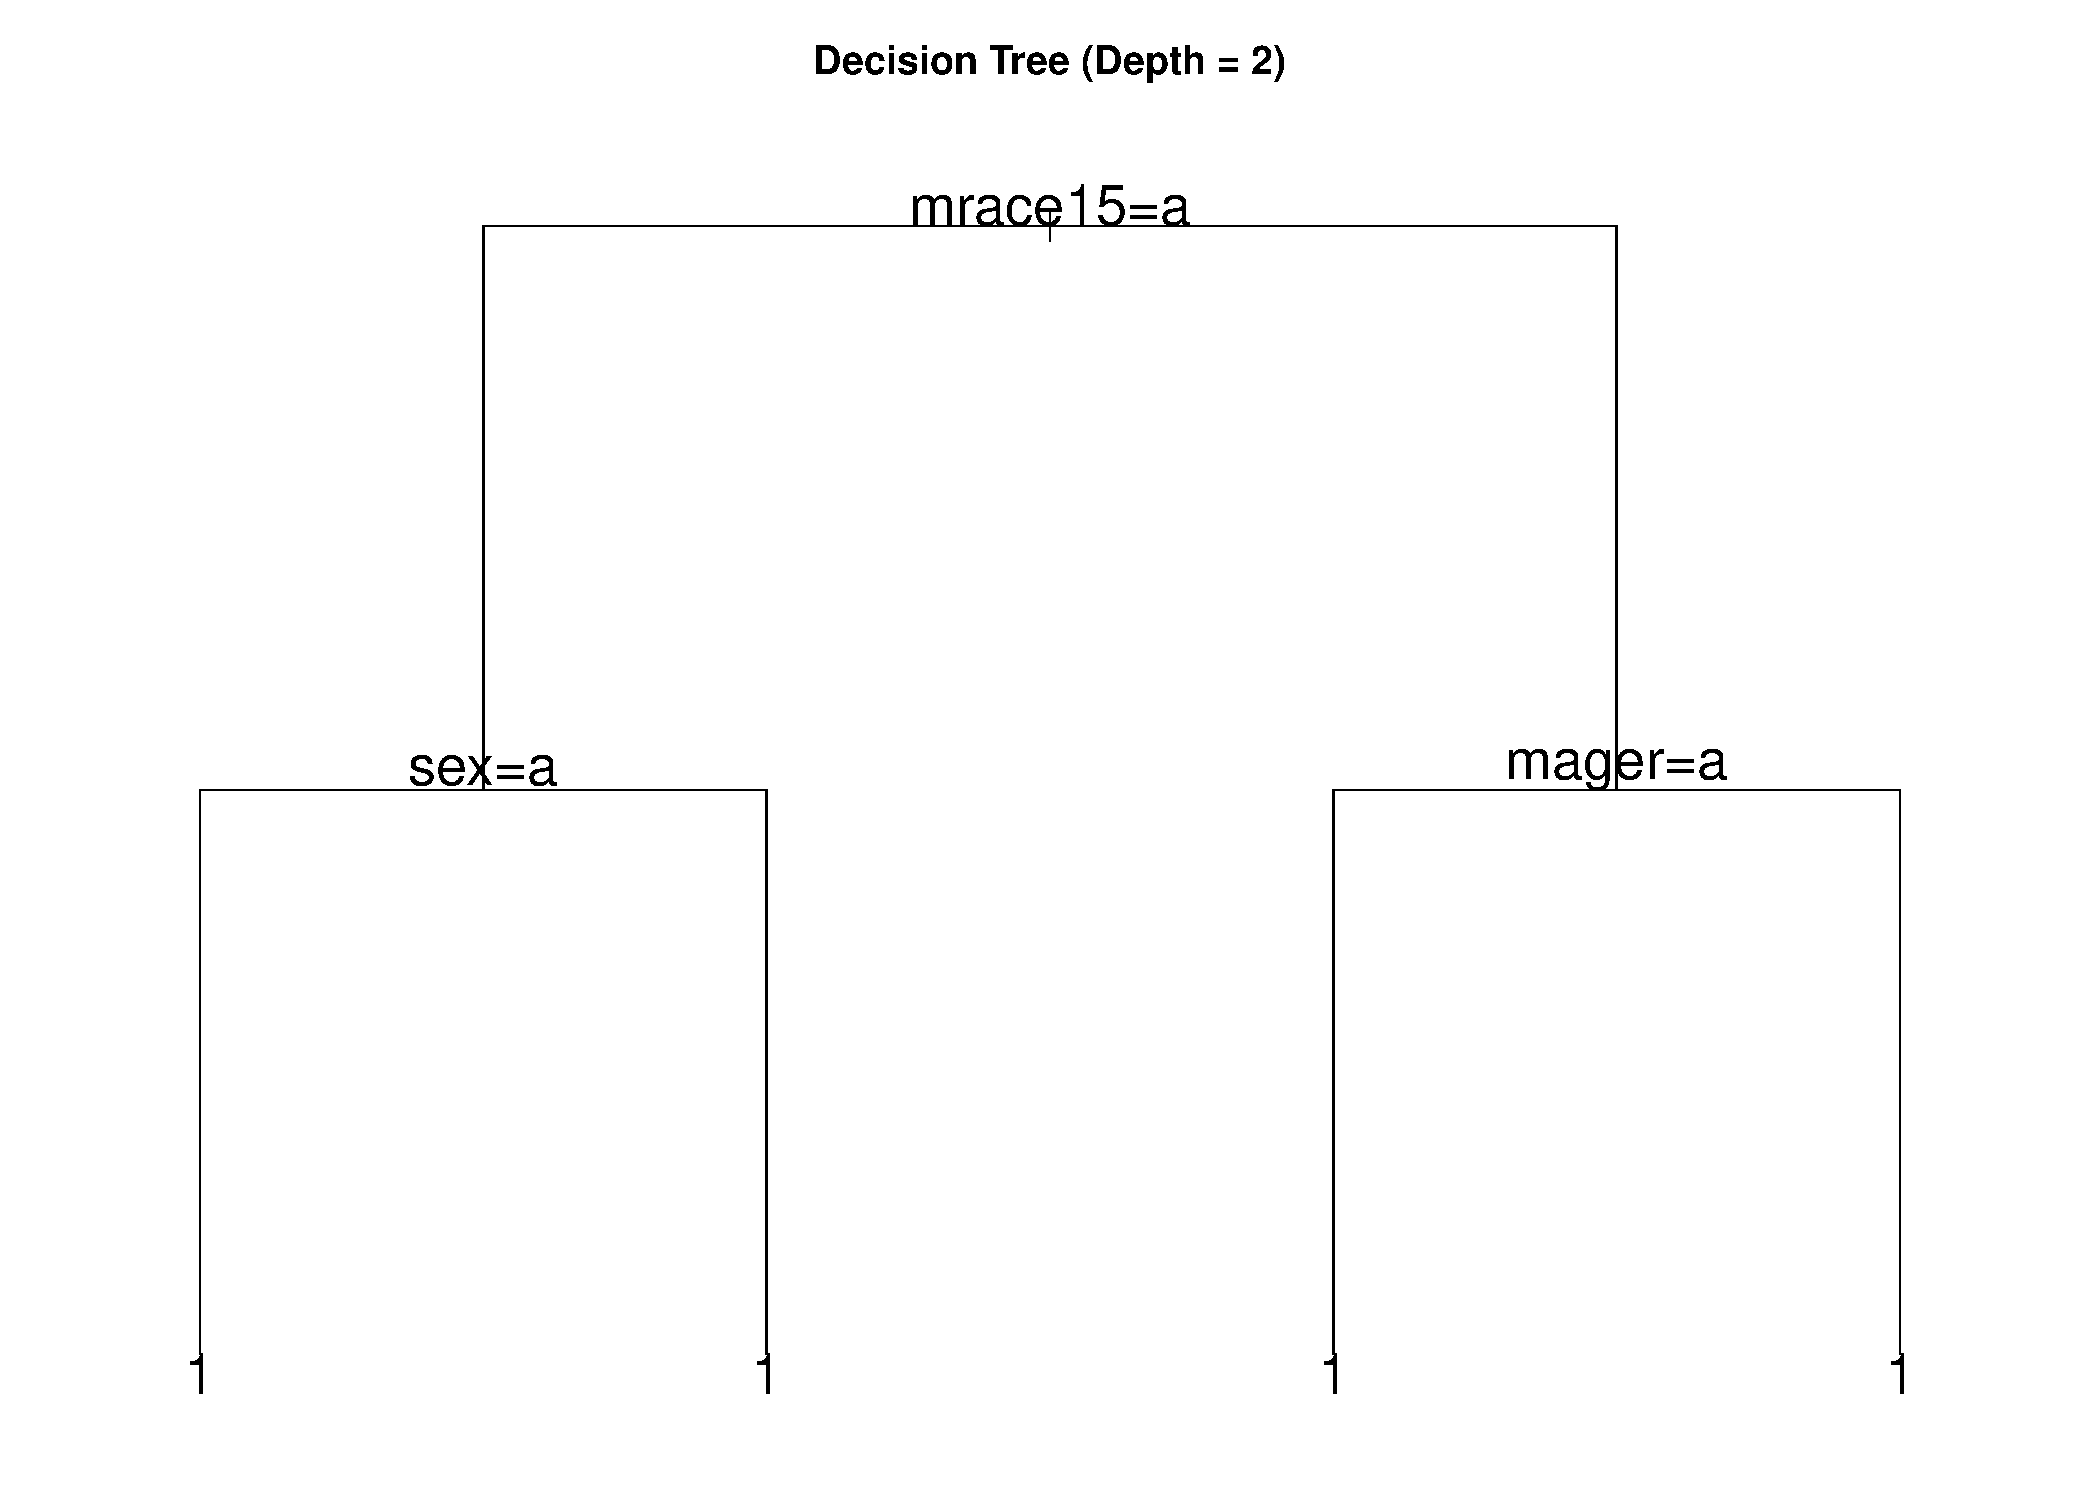
\includegraphics[width=\linewidth]{chapters/chapter3/figures/depth/plot2/decision_tree_depth_2_2021_large.pdf}
        \caption*{Maximum depth = 2}
    \end{minipage}
    \hspace{0.02\textwidth}
    \begin{minipage}{0.48\textwidth}
        \centering
        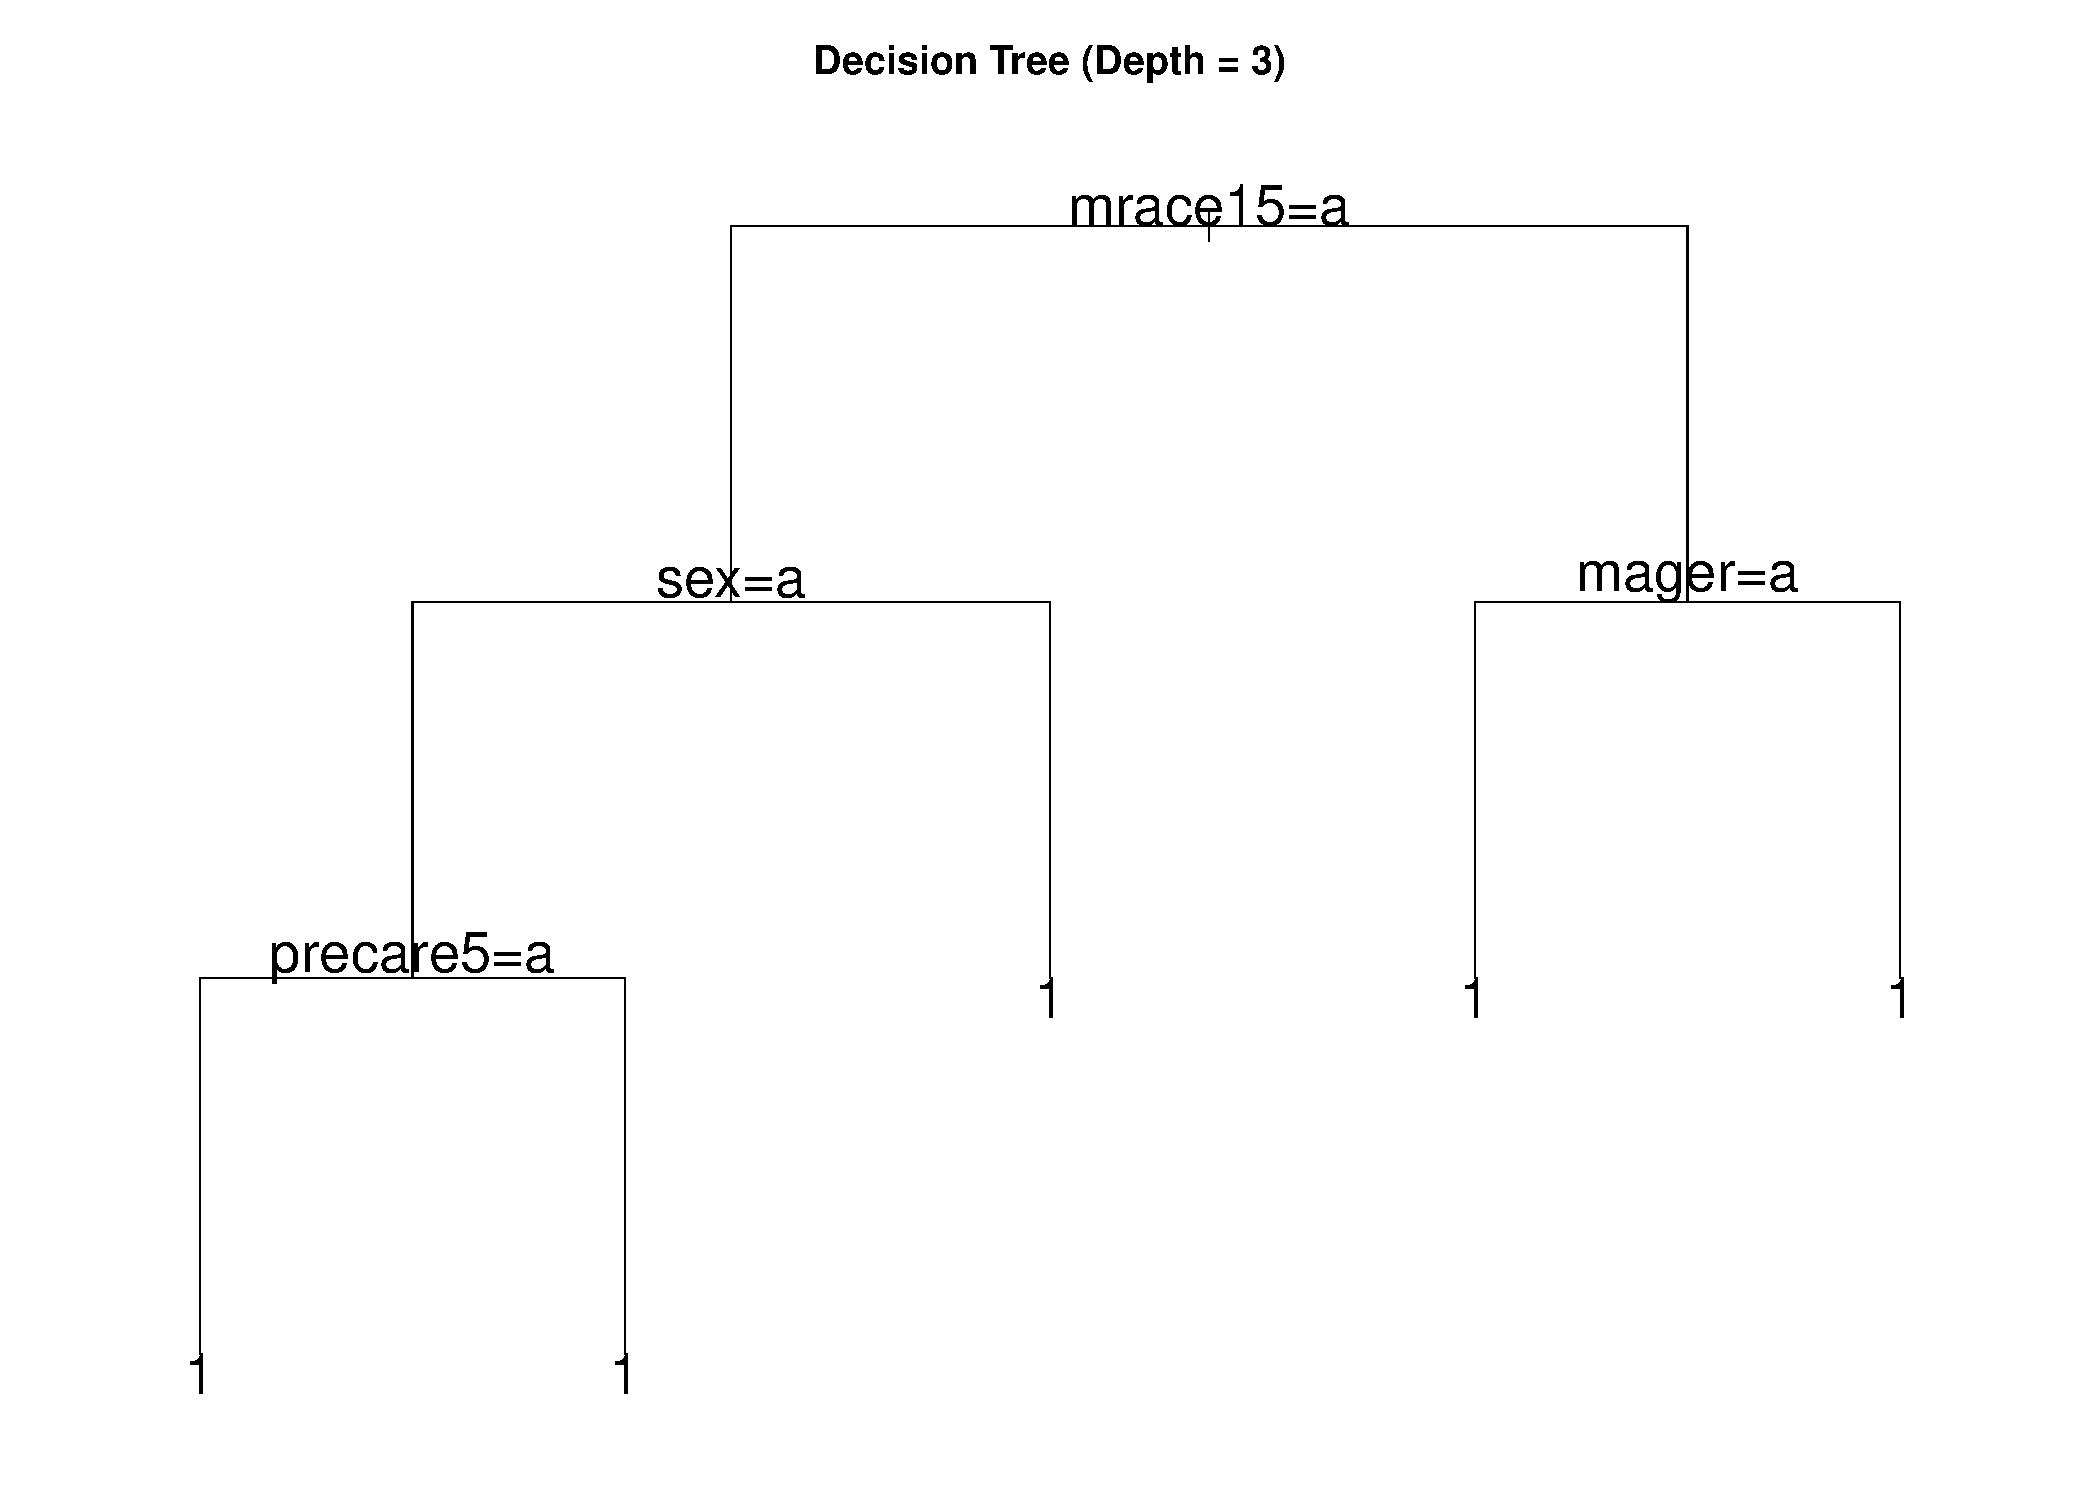
\includegraphics[width=\linewidth]{chapters/chapter3/figures/depth/plot2/decision_tree_depth_3_2021_large.pdf}
        \caption*{Maximum depth = 3}
    \end{minipage}
    
    \vspace{1cm}
    
    % Second row
    \begin{minipage}{0.48\textwidth}
        \centering
        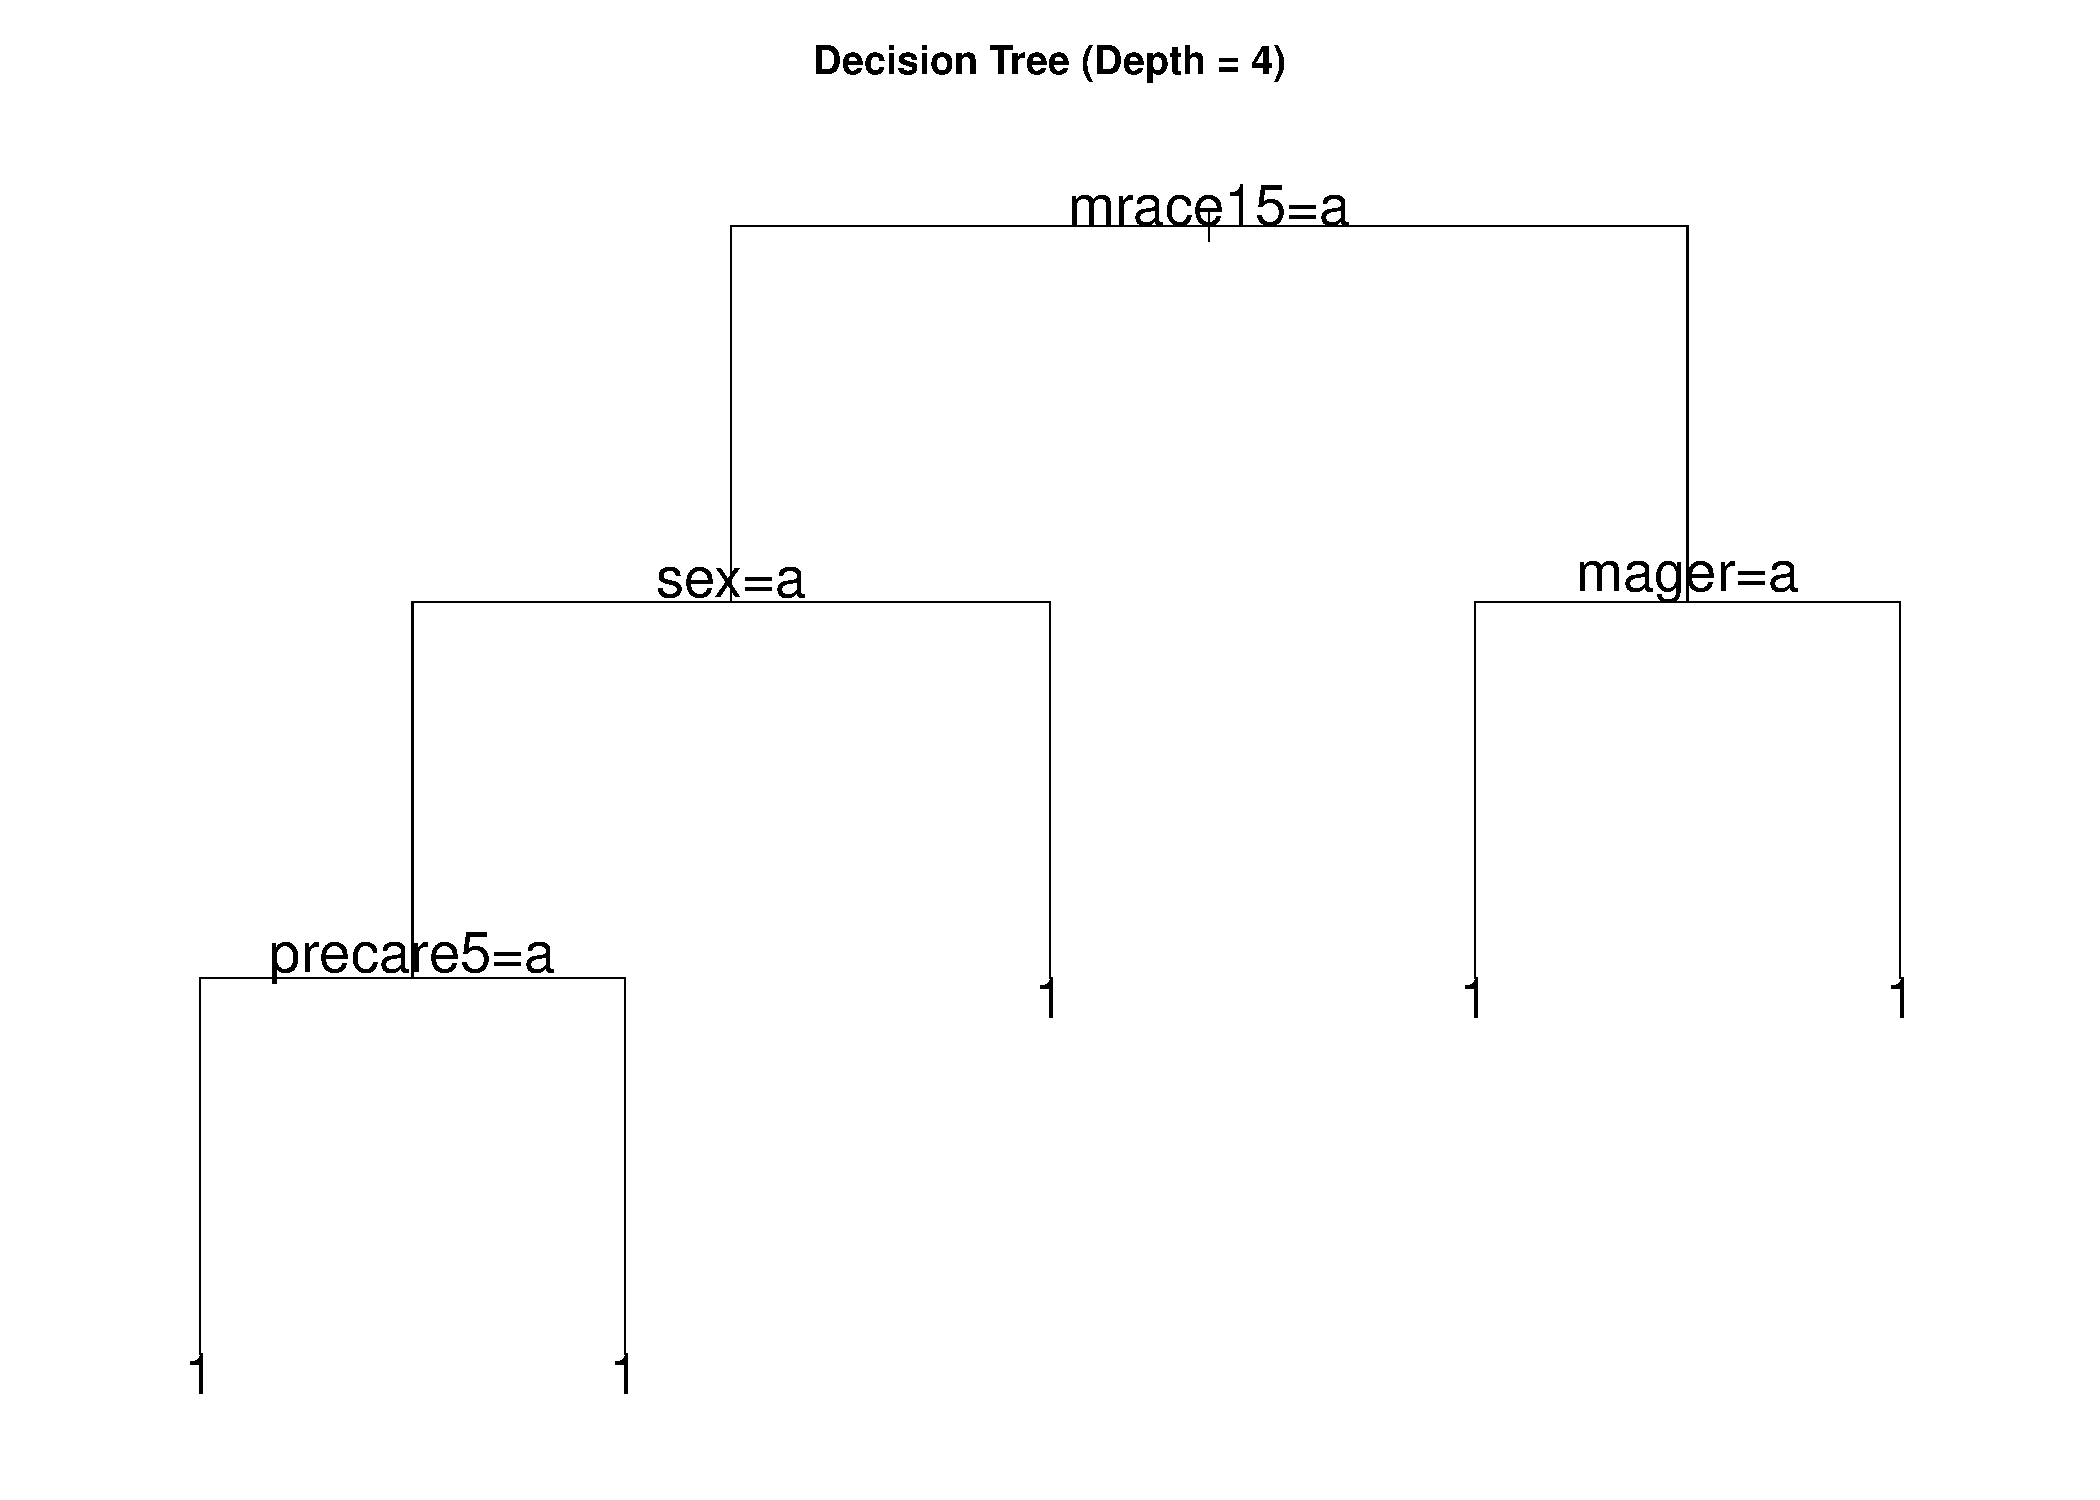
\includegraphics[width=\linewidth]{chapters/chapter3/figures/depth/plot2/decision_tree_depth_4_2021_large.pdf}
        \caption*{Maximum depth = 4}
    \end{minipage}
    \hspace{0.02\textwidth}
    \begin{minipage}{0.48\textwidth}
        \centering
        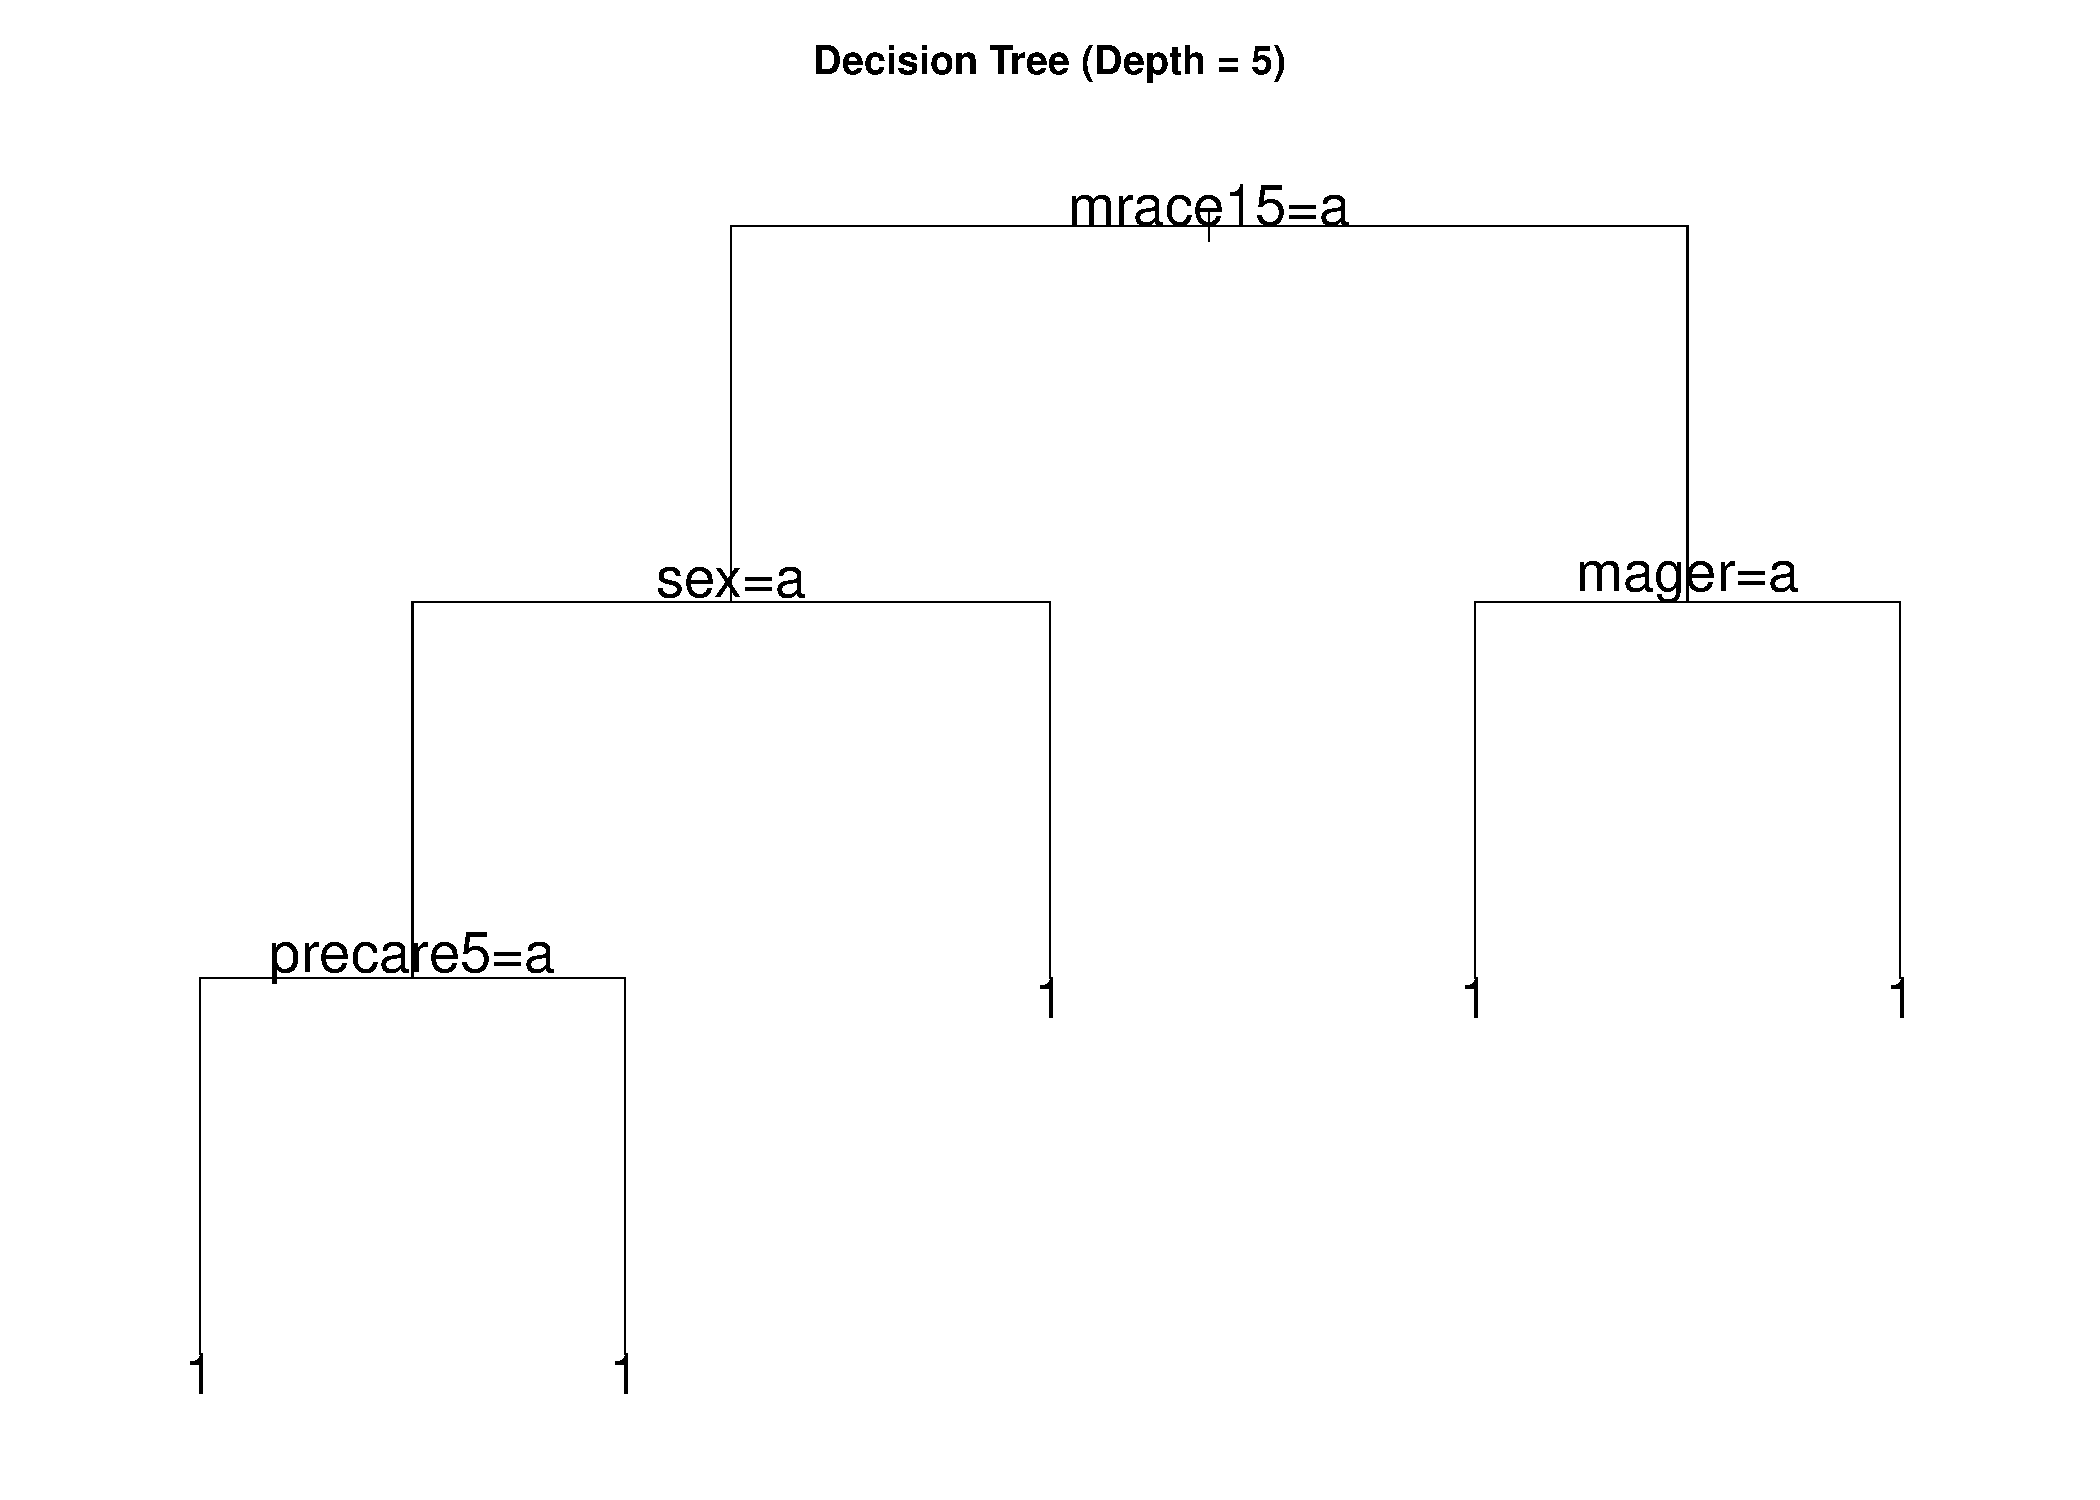
\includegraphics[width=\linewidth]{chapters/chapter3/figures/depth/plot2/decision_tree_depth_5_2021_large.pdf}
        \caption*{Maximum depth = 5}
    \end{minipage}
    \caption{LBW-only model tree structures, showing growth patterns at different maximum depths (2,3,4,5). The trees demonstrate variable selection patterns with increasing depth, highlighting the limited growth among LBW outcomes.}
    \label{fig:trees-comparison-lbw}
\end{figure}

\newpage 

\section{Bootstrap Analysis \& Methodology}
\label{sec:ch3:boot}

\subsection{Introduction}
\label{sec:ch3-boot-intro}
To test whether the splits observed in Section~\ref{sec:ch3-dm-cart} are specific to one realization of the 2021 data, we construct an ensemble of \(B =10,000\) parametric bootstrap trees. For each replicate, resampling perturbs the data into two levels, mirroring the sampling hierarchy in the DM model. That is to say, we will focus on (1) \emph{between-class} counts and (2) \emph{within-class} counts. These steps will be the stages, or tiers, of the bootstrap procedure. First, we randomize how the total number of births \(T\) is partitioned across the \(N=128\) predictor classes and secondly, given the total class partitions, we randomize how those births are allocated among the \(K\) birth-weight categories. This will deliver uncertainty estimates that are coherent with our criterion used to fit each tree. Throughout, "row" and "class" are synonymous. 

The goal of the bootstrap procedure is to provide robust and stable probability estimates \(\hat{\pi}_{i,k}\) for each category \(k\). The frequencies in Table~\ref{tab:var_comparison} therefore have a defensible interpretation as the bootstrap probabilities of variable inclusion.

\subsection{Justification of the Two-Tier Bootstrap Procedure}
\label{sec:ch3-justifiaction}
To motivate the multinomial assumption in each tier, consider the consolidated counts data. It is an \emph{aggregated} \(N \times K\) matrix where the cell entries \(n_{i,k}\) are sums of total number of births for class \(i\) and category \(k\). These sums are not \emph{individual} observations. Treating the row vector \(\mathbf{y}_i\) as an i.i.d. "case" would breech the key independence assumption that underpins case-resampling \parencite[slide 47]{case_resampling} \parencite{math10244671}. Moreover, the counts data holds the same structure as a contingency table: conveying the frequencies of any two multivariate vectors, in this case class profiles by birth-weight categories \parencite{wiki:contingency}. De-aggregating these frequencies into individual observations before performing bootstrap resampling is required to preserve the within-row dependence, preserving the data structure \parencite{stackexchangeBootstrapResampling}, precisely because each row is a vector of summary statistics (i.e. sum of total row observations) \parencite{wiki:summary_statistic}. Further, when sampling any row, the counts vector has fixed proportions of LBW and NBW counts, thereby providing no within-row randomness. Since NBW proportion greatly exceeds that of the LBW counts this would greatly overshadow the LBW variability.

When individual birth records cannot be recovered, the solution is a model-based \emph{parametric} bootstrap that respects both levels of randomness while maintaining faithful to the DM model introduced in Section~\ref{sec:ch3-prior}.

\subsection{Methodology \& Procedure}
\label{sec:ch3-boot-method}
Formally, the two-tier bootstrap resampling procedure is defined here. First, \(T\) defines the grand total counts. \(\mathbf{p} = (p_1, \dots, p_N)\) are the empirical proportions across \(N\) classes. The \emph{bootstrap probability estimates} for class \(i\)  across \(K\) categories are represented as, \(\boldsymbol{\hat{\pi}}_i = (\hat{\pi}_{i,1}, \dots,\hat{\pi}_{i,K})\), and are the mean across the \(B\) bootstrap replicate trees. Additionally, the predictor matrix \(\mathbf{X}\) remains fixed; only response counts are resampled.

\[
\begin{aligned}
T            &= \sum_{i=1}^{N}\sum_{k=1}^{K} n_{ik}              &&\text{(grand total of births)},\\[2pt]
N_i          &= \sum_{k=1}^{K} n_{ik}                            &&\text{(row total for class \(i\))},\\[2pt]
p_i          &= \frac{N_i}{T}, \qquad
\mathbf{p}   =(p_1,\dots,p_N)                                    &&\text{(empirical class shares)},\\[2pt]
\hat{\boldsymbol{\pi}}_i &= (\hat{\pi}_{i,1},\dots,\hat{\pi}_{i,K}) &&\text{(posterior DM mean for class \(i\))}.
\end{aligned}
\]

Recall that the posterior distribution in Equation~\ref{eq:closed-form} for class \(i\) is:
\[
    \boldsymbol{\theta}_i \mid \mathbf{y}_i, \mathbf{x}_i
    \;\sim\;    \operatorname{Dirichlet}\!\bigl(\boldsymbol{\alpha}+\mathbf{y}_i\bigr),
    \tag{\ref{eq:closed-form}}
\]

whose mean is:

\[
\hat{\pi}_{i,k}
\;=\;
\mathbb{E}\bigl[\theta_{i,k}\mid\mathbf{y}_i\bigr]
=
\frac{n_{ik}+\alpha_k}{N_i+\alpha_0},
\qquad
\alpha_0=\sum_{k=1}^{K}\alpha_k.
\]
All \(\hat{\pi}_{i,k}\) represent the mean bootstrap probability estimates (across \(B\)) for combination \(i,k\). Importantly, these \(K\) estimates are fixed. Instead of directly inferring about \(\theta_{i,k}\) under the posterior, we use the shrinkage estimate \(\hat{\pi}_{i,k}\). This is referred to as fixed under the multinomial distribution in Tier~\ref{para:tier-2} \cite{wiki:shrinkage_statistic, duke}. 

\paragraph{Tier 1: Between-class counts resampling}
\label{para:tier-1}
First we draw a new vector of class totals from a multinomial distribution, sampling once per class. This tier propagates sampling noise in relative prevalence of the \(N\) predictor profiles.
\begin{equation}
    \label{eq:stage1}
    \mathbf{n}_i^\ast = (n_1^\ast, \dots, n_N^\ast) \sim \mathrm{Multinomial}(T, \mathbf{p})
    \end{equation}
\paragraph{Tier 2: Within-class counts resampling}
\label{para:tier-2}
Conditioned on the newly drawn total \(n_i^\ast > 0\), resample the \(K\) category counts. 
\begin{equation}
    \label{eq:stage2}
        \tilde{\mathbf{y}}_i = (\tilde{n}_{i,1}, \dots, \tilde{n}_{i,K}) \sim \mathrm{Multinomial}(n_i^\ast, \hat{\boldsymbol{\pi}}_i)
\end{equation}
Since \(\boldsymbol{\hat{\pi}}_i = (\hat{\pi}_{i,1}, \dots,\hat{\pi}_{i,K})\) is plugged-in and held fixed here, each vector \(\hat{\boldsymbol{\pi}}_i\) under class \(i\) is referred to as the bootstrap probability estimates for \(K\) birth-weight categories. Each bootstrap replicate inherits prior information via \(\boldsymbol{\alpha}\), allowing both inter- and intra-class sampling variability to be propagated. The estimates are interpreted naturally as the best guess for the probability of a future birth from class \(i\) to fall into category \(k\). 

After the resampled counts are obtained, \(\tilde{\mathbf Y} =[\tilde n_{i,k}]\) is paired with \(\mathbf{X}\) and fitted with the DM–CART procedure.  From each tree we record the predictor set used in splitting and the root split predictor. Aggregating across \(B\) bootstrap trees yields the frequencies reported in Table~\ref{tab:var_comparison} and the predictor depth comparison in Figures~\ref{fig:var-depth-distributions-full}, ~\ref{fig:var-depth-distributions-lbw}. By tier 1 capturing the uncertainty in class prevalence, and tier 2 capturing uncertainty of the proportions of LBW and NBW within each class, these frequencies can be interpreted as the bootstrap probability of variable inclusion under the DM hierarchy. 

For each class \(i\), we compute the mean bootstrap probability estimates in \(\hat{\boldsymbol{\pi}}_i\) and hold this vector as fixed when we generate the replicate counts \(\tilde{\mathbf{y}}_i \sim \mathrm{Multinomial}(n^\ast,\hat{\boldsymbol{\pi}}_i)\). Rather than resampling a new \(\boldsymbol{\theta}_i^{(b)} \sim \mathrm{Dirichlet}(\boldsymbol{\alpha} + \mathbf{y}_i)\) inside every bootstrap replicate \(b\), we use the mean estimates and keep the resampling procedure focused on sampling variability of the observed counts data. This approach eliminates the need for a Monte-Carlo procedure and prior information \(\boldsymbol{\alpha}\) from being counted twice.

\subsection{Variable Selection Frequency}
\label{ch3:boot-var-selection}
Table~\ref{tab:var_comparison} distills the frequency of variable selection across the bootstrap ensemble. These are the probability estimates for variable inclusion under each model, highlighting the relative importance under each context. In both the full model and LBW-only model, maternal race consistently emerges as the dominant predictor, appearing as the initial split variable in 100\% of the bootstrap trees. This finding reinforces the conclusion drawn in earlier analyses (see Section~\ref{sec:ch3-comparison-depth}) that racial disparities represent the most prominent signal in the data. Figures~\ref{fig:var-depth-distributions-full} and ~\ref{fig:var-depth-distributions-lbw} show the distribution of each predictor's depth for the full and LBW-only model respectively. 

Beyond race, the variable selection patterns diverge considerably between the two models. In the full model, six of seven variables (infant gender, marital status, prenatal care, smoking status, and race) are selected in every tree (100\%), while education status is selected in approximately 37.94\% of the ensemble. Despite its relatively lower selection frequency, maternal education is deeply positioned in the trees, with an average depth of 5.52 in Figure~\ref{fig:var-depth-distributions-full}, suggesting weak but possibly contextually relevant role in specific subpopulations. In contrast, marital status and smoking status appear much closer to the root at depths 1.69 and 1.52 respectively, indicating stronger global influence across the data. 

In the LBW-only model, the frequency and depth of variable inclusion reflects the shift of model focus. While race and infant gender remain universally selected (100\%), only maternal age maintains high inclusion at 97.41\%, and prenatal care follows at 63.51\%. The remaining variables occur rarely or not at all with marital status (9.15\%), smoking status (1.96\%), and maternal education (0\%). The stark drop in inclusion frequency suggests that given the LBW outcomes, the model reduces its reliance on broader social determinants like education and marital status, and concentrates on variables more directly related to biological and perinatal features such as age and care access. 

This interpretation is further supported by the depth analysis in Figures~\ref{fig:var-depth-distributions-full},~\ref{fig:var-depth-distributions-lbw}. For LBW-only model, maternal race is the top splitter, followed by infant sex (mean depth of 1.12), maternal age (1.15), indicating the early and consistent splits. Prenatal care appears at an intermediate depth (2.02) and less frequently included variables exhibit greater depth, such as marital status and smoking status (2.83 and 2.94, respectively). Notably, maternal education with negligible frequency and high depth (3.00), emphasizing minimal contribution in LBW context. 


\subsection{Ensemble Predictions \& Uncertainty}
\label{sec:ch3-boot-pred}

Following the bootstrap resampling procedure, each replicate yields a vector of predicted probabilities in \(\tilde{\mathbf{Y}}\) for the birth-weight categories aggregated across \(B\). For every terminal node subgroup, we take the mean across all replicates to obtain \(\hat{\pi}_{i,k}\): the estimated probability that a birth in class \(i\) falls into birth-weight category \(k\). Sampling variability is summarized by empirical 2.5- and 97.5-percentiles of each birth-weight category distribution. These 95\% percentile intervals are shown along side point estimates in Tables~\ref{tab:pi_mean_full} and ~\ref{tab:pi_mean_lbw}. Because the interval is simply the middle 95\% of the resampled values, it is distribution-free \parencite{percentile-interval}.  For some \(i,k\) combination, the interval is read as 2.5\% (or 97.5\%) of replicates assign smaller (larger) probability than the reported limit \parencite{percentile-interval}. Figures~\ref{fig:high-low-risk-full} and~\ref{fig:high-low-risk-lbw} display the full distribution of two contrasting maternal profiles.  Such profiles are referred to as "high-risk" (class 69) and "low-risk" (class 28) and reflect reasonably assumed to face adverse and favorable birth-weight outcomes, respectively.

\begin{itemize}
  \item \emph{High‑risk} (\(i=69\)): unmarried, Black, smoking mothers under 33 with $<$ High-School education, inadequate prenatal care, delivering female infants (\texttt{mrace15} = 1, \texttt{dmar} = 0, \texttt{cig\_0} = 1, \texttt{sex} = 0, \texttt{mager} = 0, \texttt{prenatal} = 0, \texttt{meduc} = 0).
  \item \emph{Low‑risk} (\(i=28\)): married, non‑Black, non‑smoking mothers aged 33+, $\geq$ High-School education, adequate prenatal care, delivering male infants (\texttt{mrace15} = 0, \texttt{dmar} = 1, \texttt{cig\_0} = 0, \texttt{sex} = 1, \texttt{mager} = 1, \texttt{prenatal} = 1, \texttt{meduc} = 1).
\end{itemize}

In the full model, Figures~\ref{fig:high-low-risk-full}, \ref{fig:high-low-risk-full-w/o-NBW} and Table~\ref{tab:pi_mean_full}. Specifically, in Figure~\ref{fig:high-low-risk-full} we see that both profiles have a very high predicted probability of delivering a NBW infant, yet this high-risk’s NBW chance (83.6\%) is roughly 7\% points lower than the low-risk profile (90.9\%). In Figure~\ref{fig:high-low-risk-full-w/o-NBW} we focus on the probabilities within LBW-region under the full model. This diagram shows the drastic differences of risk among the high- and low-risk profiles, with an average probability of 1.64\% versus 0.908\%, respectively. For the most severe LBW category (C1 or \(k=1\)), the highest probability is triple that of the low-risk subgroup (1.9\% vs. 0.8\%). The percentile intervals are extremely narrow (\(\approx \pm 0.002\)) indicating remarkable stability across all bootstrap replicates. 

Likewise, the LBW-only model in Figure~\ref{fig:high-low-risk-lbw} and Table~\ref{tab:pi_mean_lbw}, provides more nuance among the LBW region. The high-risk profile retains a clear disadvantage in the extreme left-tail (12.3\% vs. 8.6\% in C1), but the two subgroups converge in the intermediate categories, and in a few moderate LBW categories the low-risk profile even slightly exceeding high-risk subgroup (such as in C8 or \(k=8\) of Table~\ref{tab:pi_mean_lbw}). Percentile interval widths still remain narrow (\(\approx \pm 0.008\)), illustrating that these nuanced differences are nonetheless estimated with high stability and precision. 

In identifying determinants of LBW outcomes, this procedure clearly delineates a consistent and statistically reliable separation between high- and low-risk profiles, even when the absolute differences in NBW probabilities appears modest.
